% =============================================================================
%  CHƯƠNG 4 – KẾT QUẢ MÔ PHỎNG VÀ ĐÁNH GIÁ
% =============================================================================
\chapter{KẾT QUẢ MÔ PHỎNG VÀ ĐÁNH GIÁ}
\label{ch:chuong4}

Chương này trình bày kết quả mô phỏng số học để đánh giá hiệu năng của
khuôn khổ MADDPG-CTDE đề xuất so với các thuật toán DRL tham chiếu và các
phương pháp xử lý STAR-RIS truyền thống. Các kết quả được phân thành các
nhóm: (1) thiết lập mô phỏng (mục \ref{sec:setup}), (2) hội tụ huấn
luyện (mục \ref{sec:convergence}), (3) so sánh thuật toán DRL (mục
\ref{sec:algo_comp}), (4) độ nhạy với công suất phát (mục \ref{sec:power_sweep}),
(5) khả năng mở rộng theo số phần tử STAR-RIS (mục \ref{sec:scalability}),
(6) phân tích loại trừ cho STAR-RIS (mục \ref{sec:ablation}) và (7) phân
tích chuyên sâu (mục \ref{sec:deep_analysis}).

\noindent\fbox{\parbox{0.97\linewidth}{\small\textbf{Ghi chú về nguồn số
liệu (bản nháp --- PENDING).} Các con số trong chương này được sinh bởi
pipeline mô phỏng phiên bản trước refactor 2026-07-16 (formulation
block-fading tĩnh trong episode, chỉ số QoS đo ``tất cả người dùng đồng
thời đạt ngưỡng'', baseline AO-Grid khi đó bị gọi là BCD, vùng tin cậy
của hình hội tụ tính bằng rolling std). Toàn bộ bảng và hình của chương
sẽ được tái sinh bằng pipeline Dynamic-MDP mới (mô tả ở Chương 2--3)
theo quy trình trong \texttt{KAGGLE\_RERUN\_CHECKLIST.md}; kết quả cũ
được lưu tại \texttt{results\_legacy/} và không dùng làm bằng chứng
cuối cùng. Các định nghĩa metric và cách tính thống kê nêu dưới đây là
của pipeline mới.}}

% -----------------------------------------------------------------------------
\section{Thiết lập mô phỏng}
\label{sec:setup}

\subsection{Tham số hệ thống và phần cứng}

Hệ thống STAR-RIS RSMA được mô phỏng bằng Python 3.10 với PyTorch 2.x.
Bảng \ref{tab:simulation_parameters} liệt kê toàn bộ tham số mô phỏng,
được trích xuất tự động từ tệp cấu hình \texttt{config.yaml} của thư
viện mã nguồn để đảm bảo tính tái lập.

\begin{table}[t]
\centering
\small
\caption{Tham số mô phỏng đầy đủ của hệ thống và thuật toán.}
\label{tab:simulation_parameters}
\begin{tabular}{ll}
\toprule
\textbf{Tham số} & \textbf{Giá trị} \\
\midrule
\multicolumn{2}{l}{\textbf{Cấu hình hệ thống}} \\
Số người dùng tổng ($K$) & 4 \\
Số người dùng vùng phản xạ ($K_R$) & 3 \\
Số phần tử STAR-RIS ($N$) & 32 \\
Số anten BS ($M$) & 4 \\
Công suất phát tối đa $P_{\max}$ & $30$ dBm \\
Công suất tạp âm $\sigma^2$ & $-90$ dBm \\
QoS tối thiểu $R_{\min}$ & $0{,}3$ b/s/Hz \\
Suy hao chướng ngại UE$_T$ & $25$ dB \\
Số mũ suy hao kênh trực tiếp $\alpha_d$ & $3{,}5$ \\
Số mũ suy hao kênh BS-RIS $\alpha_G$ & $2{,}2$ \\
Số mũ suy hao kênh RIS-UE $\alpha_r$ & $2{,}5$ \\
\midrule
Hệ số tương quan kênh Gauss--Markov $\rho$ & $0{,}95$ \\
\midrule
\multicolumn{2}{l}{\textbf{Tham số hàm phần thưởng (Lagrangian surrogate)}} \\
Hệ số $\alpha$ sum-rate / $R_{\text{ref}}$ & $1{,}5$ / $20$ b/s/Hz \\
Trọng số augmented penalty $w$ & $1{,}0$ \\
$\lambda_k$ ban đầu / miền chiếu & $1{,}0$ / $[0,\,20]$ \\
Tốc độ học đối ngẫu $\eta_\lambda$ / EMA & $0{,}01$ / $0{,}9$ \\
Tỷ lệ đóng băng $\lambda$ ($\rho_f$) & $0{,}55$ \\
Trọng số switching cost $\eta_\phi/\eta_P/\eta_\beta$ & $0{,}1$ / $0{,}05$ / $0{,}05$ \\
Ánh xạ pha mặc định & Pha tuyệt đối, $\phi_n=\pi(a_n+1)$ \\
\midrule
\multicolumn{2}{l}{\textbf{Tham số huấn luyện}} \\
Số episode mỗi thuật toán & $2\,000$ \\
Số hạt giống huấn luyện & $8$ (cấu hình chuẩn và sweep $N$) \\
Hạt giống validation / test (khóa) & $[11,\ldots,55]$ / $[70001,\ldots,70005]$ \\
Nguồn seed split / SHA-256 & \texttt{seed\_split.v1.yaml} / \texttt{d73ba5aea6d0\ldots f118854} \\
Số bước warmup ngẫu nhiên & $5\,000$ \\
Mốc đóng băng normalizer quan sát & $5\,000$ bước môi trường \\
Số bước decay nhiễu OU & $45\,000$ \\
\bottomrule
\end{tabular}

\vspace{0.2em}
\hfill {\footnotesize\itshape Nguồn: Tác giả xây dựng (2026)}
\end{table}


\subsection{Các baseline được so sánh}

Để đánh giá khách quan, MADDPG đề xuất được so sánh với tám baseline,
chia làm hai nhóm:

\noindent\textbf{Nhóm A, Các thuật toán DRL đơn tác tử / đa tác tử khác:}
\begin{itemize}[leftmargin=*]
\item \textbf{DDPG} \cite{lillicrap2016continuous}: tác tử đơn với hành
động 140 chiều hợp nhất.
\item \textbf{TD3} \cite{fujimoto2018addressing}: cải tiến của DDPG với
hai Critic và trì hoãn cập nhật Actor.
\item \textbf{PPO} \cite{schulman2017proximal}: thuật toán on-policy với
clip surrogate objective.
\end{itemize}

\noindent\textbf{Nhóm B, Các phương pháp xử lý STAR-RIS truyền thống:}
\begin{itemize}[leftmargin=*]
\item \textbf{AO-Grid}: heuristic tối ưu xen kẽ dạng lưới thô
(coarse alternating-optimization grid): pha lấy nghiệm phân tích căn
đồng pha cho người dùng yếu nhất, một hệ số $\beta$ chung cho mọi phần
tử tìm trên lưới 5 điểm, tỷ lệ $P_c/P_{\max}$ tìm trên lưới 6 điểm,
công suất riêng và tỷ lệ tách chia đều. Đây là một \emph{heuristic tham
chiếu}, không phải cận trên tối ưu và không xử lý ràng buộc QoS.
(Trong pipeline cũ phương pháp này bị gọi nhầm là ``BCD/cận trên''.)
\item \textbf{Hybrid AO Local Search} (SLSQP + projected gradient): tìm
kiếm cục bộ xen kẽ trên đúng không gian biến của P0 (vector
$\beta_n^R$ per-element, pha, công suất, tỷ lệ tách), đa điểm khởi
tạo, cùng hàm mục tiêu surrogate và chi phí tái cấu hình như DRL;
chạy cho $N \leq 32$. Là mốc tham chiếu tìm kiếm cục bộ, không phải
cận trên.
\item \textbf{MaxMinAligned}: căn pha đồng pha cho người dùng yếu nhất,
sử dụng công thức \eqref{eq:phase_prior} mà không có RL tinh chỉnh.
\item \textbf{FixedRIS}: $\beta_n^R = \beta_n^T = 1/2$, $\theta_n^X = 0$ cho
mọi $n$.
\item \textbf{RandomRIS}: pha ngẫu nhiên đều trong $[0, 2\pi)$ cho mọi
phần tử, biên độ ngẫu nhiên trong $[0,1]$.
\item \textbf{NoRIS}: bỏ STAR-RIS, chỉ giữ kênh trực tiếp $h_{d,k}$.
\end{itemize}
Nhóm A còn bổ sung \textbf{TD3-Matched}: TD3 đơn tác tử với bề rộng lớp
ẩn được chọn tự động sao cho \emph{tổng} tham số khả huấn luyện khớp
MADDPG trong sai lệch $5\%$, dùng để tách bạch lợi ích của phân rã đa
tác tử khỏi lợi ích thuần túy về dung lượng mạng.

\subsection{Phương pháp đánh giá}

Tất cả các kết quả tại cấu hình chuẩn $N=32$ được lấy trung bình trên
$8$ hạt giống huấn luyện độc lập $\{1000, 2000, \ldots, 8000\}$; đơn vị
phân tích thống kê là \emph{trung bình theo hạt giống huấn luyện}: mỗi
hạt giống được đánh giá xác định (deterministic) trên cùng một tập kịch
bản kiểm tra đã khóa (ScenarioBank: hình học người dùng, kênh khởi tạo
và chuỗi innovation Gauss--Markov sinh trước, giống hệt nhau cho mọi
phương pháp), rồi khoảng tin cậy $95\%$ Student-t được tính qua $8$ giá
trị trung bình đó. Các baseline không học (AO-Grid, MaxMinAligned,
FixedRIS, \ldots) không phụ thuộc hạt giống huấn luyện nên độ bất định
của chúng được tính qua các kịch bản đánh giá độc lập. Tập hạt giống
$\{11, \ldots, 55\}$ trước đây --- đã được xem trong quá trình phát
triển --- chỉ dùng làm \emph{validation} (chọn mô hình, tinh chỉnh);
kết quả báo cáo dùng tập kịch bản kiểm tra khóa sinh từ các hạt giống
mới $\{81011, 81023, 81041, 81071, 81101\}$. Danh sách phát triển, validation,
legacy $\{9101,\ldots,9505\}$ và final-test được đăng ký duy nhất tại
\texttt{config/seed\_split.v2.yaml}, SHA-256
\texttt{dc327042efcad7007efa0006f0b10461eb69055992a3cdcd6416612d15db13e8};
pipeline từ chối chạy nếu hash không khớp. Riêng thí nghiệm khả năng mở rộng theo
$N$ (mục \ref{sec:scalability}) sử dụng $10$ hạt giống huấn luyện cho
mỗi điểm cấu hình. Kiểm định ý nghĩa thống kê dùng thiết kế theo cặp
(cùng danh sách hạt giống huấn luyện, cùng kịch bản đánh giá): paired
t-test và sign-flip permutation test trên các trung bình mức hạt
giống, hiệu chỉnh Holm--Bonferroni cho họ bốn so sánh chính
$\{$MADDPG vs TD3, TD3-Matched, DDPG, PPO$\}$ trên sum-rate; kích thước hiệu ứng
(Cohen's d theo cặp) và CI của hiệu số được báo cáo kèm (Bảng
\ref{tab:significance}).

% -----------------------------------------------------------------------------
\section{Hội tụ huấn luyện}
\label{sec:convergence}

\subsection{Đường cong hội tụ về tổng phần thưởng}

Hình \ref{fig:training_convergence} thể hiện đường cong hội tụ của tổng
phần thưởng (Return) theo episode đối với các thuật toán DRL trên
$2\,000$ episode. Mỗi đường của từng hạt giống được làm trơn riêng
(trung bình trượt), sau đó tại từng episode tính trung bình và khoảng
tin cậy $95\%$ Student-t \emph{qua $8$ hạt giống huấn luyện}; vùng tô
bóng là khoảng tin cậy giữa các hạt giống này.

\begin{figure}[t]
  \centering
  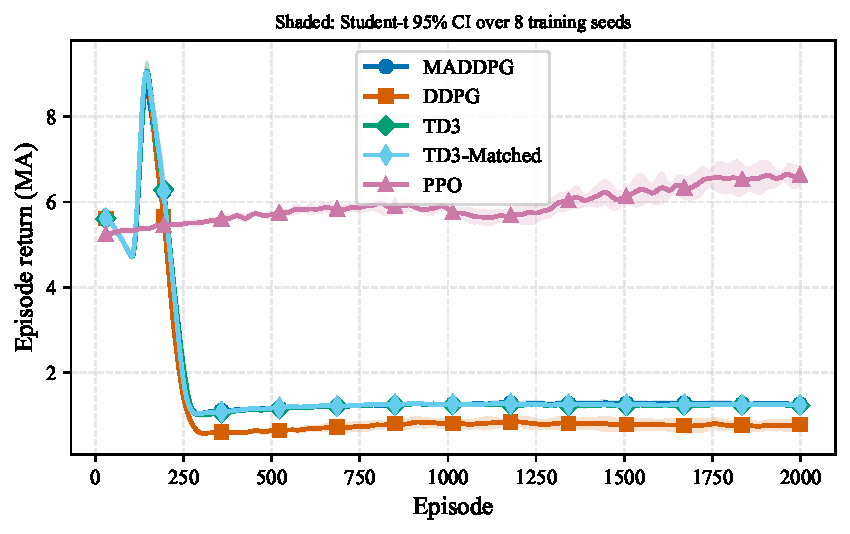
\includegraphics[width=0.85\linewidth]{figures/training_convergence.pdf}
  \caption{Đường cong hội tụ tổng phần thưởng (Return) theo episode trên
  8 hạt giống huấn luyện độc lập. Vùng bóng mờ là khoảng tin cậy $95\%$
  Student-t giữa các hạt giống (mỗi hạt giống được làm trơn riêng trước
  khi tổng hợp).}
  \label{fig:training_convergence}
\end{figure}

Có thể thấy: PPO hội tụ chậm và đều nhờ cập nhật on-policy bảo thủ.
MADDPG khởi đầu chậm do cần làm đầy replay buffer, sau đó tăng nhanh
và đạt vùng bão hòa quanh episode $700$--$1\,000$. Kể từ mốc đóng băng
$\boldsymbol{\lambda}$ (episode $1\,100$), hàm phần thưởng trở nên dừng
và các đường cong đi ngang ổn định. Lưu ý về diễn giải: vùng phẳng này
cho thấy phần thưởng đã dừng và chính sách ổn định theo thang đo đó;
nó \emph{không} tự nó chứng minh chính sách đã hội tụ về nghiệm tối
ưu.

\subsection{Tổng tốc độ qua các episode}

Hình \ref{fig:training_sum_rate} cho thấy tổng tốc độ $R_{\text{sum}}$
trung bình theo episode. Đây là chỉ số trực tiếp phản ánh mục tiêu của
bài toán P0.

\begin{figure}[t]
  \centering
  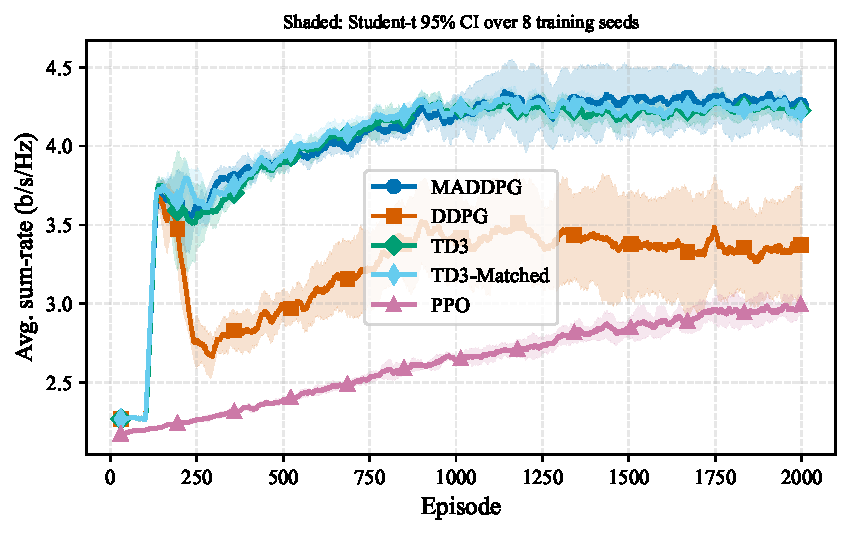
\includegraphics[width=0.85\linewidth]{figures/training_sum_rate.pdf}
  \caption{Tổng tốc độ $R_{\text{sum}}$ (b/s/Hz) theo episode trong quá
  trình huấn luyện (trung bình 8 hạt giống). MADDPG và TD3 hội tụ về
  sum-rate cao nhất và đạt trạng thái phẳng ở nửa cuối.}
  \label{fig:training_sum_rate}
\end{figure}

Ba thuật toán đạt sum-rate cao nhất sau khi hội tụ là MADDPG ($\sim 4{,}52$
b/s/Hz), TD3-Matched ($\sim 4{,}41$) và TD3 ($\sim 4{,}39$) --- gần như trùng
nhau. PPO có sum-rate thấp hơn ($\sim 3{,}42$) vì
PPO ưu tiên thỏa mãn QoS tuyệt đối (xem hình tiếp theo). DDPG đơn tác tử có
sum-rate thấp nhất ($\sim 3{,}94$); so sánh chi tiết với TD3 --- đơn tác tử mạnh
nhất --- được trình bày ở mục \ref{sec:algo_comp} và \ref{sec:scalability}.

\subsection{Xác suất thỏa mãn QoS}

Luận văn phân biệt rõ hai chỉ số QoS
(\eqref{eq:user_qos_fraction}--\eqref{eq:all_users_qos}): tỷ lệ người
dùng đạt ngưỡng (user QoS fraction) và xác suất \emph{tất cả} $K$ người
dùng đồng thời đạt ngưỡng (all-users QoS). Hình
\ref{fig:training_qos_prob} biểu diễn chỉ số theo episode trong quá
trình huấn luyện; pipeline mới vẽ cả hai chỉ số trên hai hình riêng và
mỗi hình ghi rõ metric.

\begin{figure}[t]
  \centering
  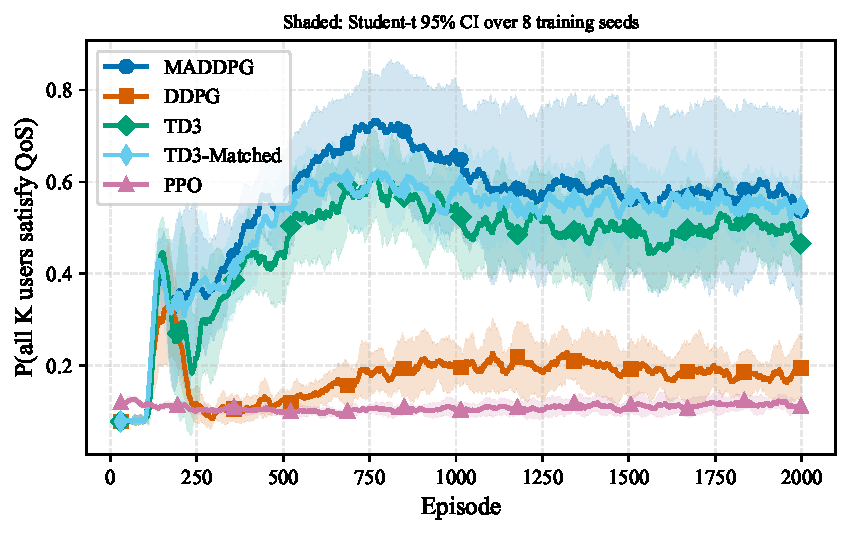
\includegraphics[width=0.85\linewidth]{figures/training_qos_prob.pdf}
  \caption{Chỉ số thỏa mãn QoS theo episode: xác suất tất cả $K=4$
  người dùng đồng thời đạt $R_{\min}$ (all-users QoS). MADDPG đạt mức
  cao nhất ($\approx 0{,}61$) tại cấu hình chuẩn $N=32$.}
  \label{fig:training_qos_prob}
\end{figure}

MADDPG đạt all-users QoS $\approx 0{,}61$ --- cao nhất trong các thuật
toán DRL tại $N=32$ --- trong khi vẫn giữ sum-rate cao nhất; cần nhấn
mạnh rằng con số này là \emph{xác suất cả bốn người dùng đồng thời đạt
$R_{\min}$} (all-users QoS), không phải tỷ lệ người dùng đạt ngưỡng ---
tỷ lệ người dùng đạt ngưỡng (QoS/UE) luôn cao hơn, với MADDPG đạt
$\approx 0{,}84$. Điểm vận hành có thể dịch chuyển thêm về phía QoS
bằng cách tăng miền chiếu $\lambda_{\max}$. Điều đó phản ánh đúng bản chất surrogate của hàm
phần thưởng: các biến đối ngẫu $\lambda_k$ điều chỉnh cân bằng giữa hai
mục tiêu, và điểm vận hành có thể dịch chuyển về phía QoS bằng cách
tăng miền chiếu $\lambda_{\max}$ (mục \ref{sec:tradeoff_discussion}).

\subsection{Sự tiến hóa của các biến đối ngẫu $\lambda_k$}

Hình \ref{fig:qos_lambda} cho thấy động học của các biến đối ngẫu theo
thời gian huấn luyện (pipeline mới ghi log từng $\lambda_k$ riêng).
Biểu đồ này giúp kiểm chứng hoạt động của cập nhật projected dual
gradient và lịch trình hai pha (two-stage dual freeze).

\begin{figure}[t]
  \centering
  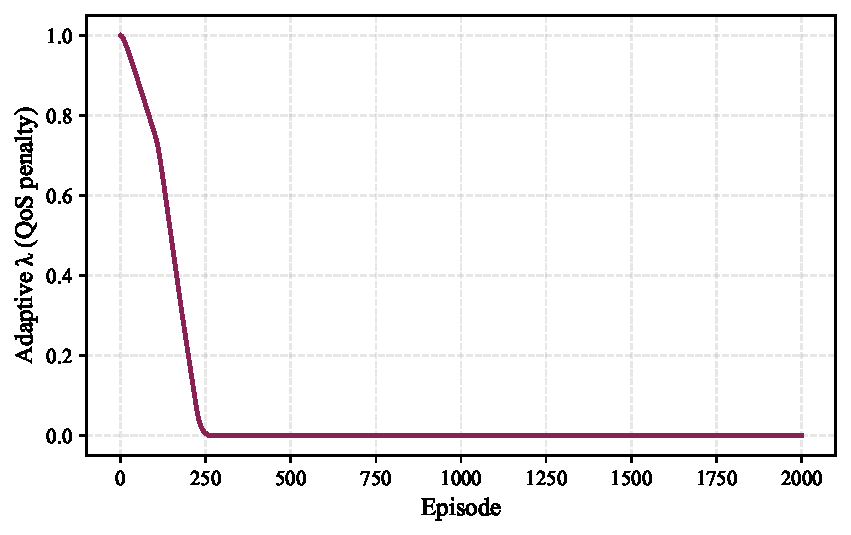
\includegraphics[width=0.85\linewidth]{figures/qos_lambda.pdf}
  \caption{Sự tiến hóa của các biến đối ngẫu $\lambda_k$ theo lịch
  trình hai pha: pha cập nhật đối ngẫu và pha đóng băng từ episode
  $1\,100$ ($55\%$ của $2\,000$ episode, phần thưởng dừng). Hình hiển
  thị vector $\lambda_k$ per-user của pipeline Dynamic-MDP.}
  \label{fig:qos_lambda}
\end{figure}

Trong pha cập nhật, $\lambda_k$ tăng khi người dùng $k$ vi phạm ràng
buộc theo kỳ vọng và giảm khi có slack (khe hở có dấu), đúng hành vi
hai chiều của gradient đối ngẫu; việc một số $\lambda_k$ bám sát biên
trên cho thấy ràng buộc QoS bó chặt với hình học kênh khảo sát.
Kể từ mốc đóng băng (episode $1\,100$), $\boldsymbol{\lambda}$ được giữ
nguyên theo \eqref{eq:lambda_freeze}: hàm phần thưởng trở nên dừng và
đường Return ở Hình \ref{fig:training_convergence} nhờ đó có thể đi
ngang.

Về cấu trúc phần thưởng: phép ánh xạ softmax của tác tử BS bảo đảm
$P_c + \sum_k P_k = P_{\max}$ theo cấu trúc nên ràng buộc (C1) tự động
được thỏa; vì lý do đó pipeline mới đã loại hẳn số hạng phạt công suất
(một số hạng luôn bằng không) khỏi hàm phần thưởng. Phần thưởng được
chi phối bởi cân bằng giữa thành phần sum-rate, thành phần đối ngẫu
QoS và chi phí tái cấu hình --- đúng như thiết kế ở Chương 3.

% -----------------------------------------------------------------------------
\section{So sánh các thuật toán DRL}
\label{sec:algo_comp}

\subsection{Bảng so sánh tổng hợp}

Bảng \ref{tab:algorithm_comparison} so sánh hiệu năng của MADDPG với
các thuật toán DRL đơn tác tử trên các chỉ số: Return, Sum-rate, xác
suất QoS, tốc độ luồng chung $R_c$, entropy pha, tỷ lệ $P_c/P_{\max}$,
độ trễ suy luận, và $\lambda$ huấn luyện cuối cùng.

\begin{table}[t]
\centering
\small
\caption{So sánh hiệu năng các thuật toán DRL trên locked test ScenarioBank tại cấu hình chuẩn $N=32$ (pipeline Dynamic-MDP; đơn vị phân tích = trung bình theo hạt giống huấn luyện, khoảng tin cậy Student-t $95\%$ qua $8$ hạt giống). Return theo tập bị lược khỏi so sánh chéo vì vector $\lambda$ tối ưu khác nhau giữa các thuật toán; các cột dưới là chỉ số vật lý. QoS all-users là $\Pr[\min_k R_k \ge R_{\min}]$; QoS/UE là $(1/K)\sum_k \mathbf{1}[R_k \ge R_{\min}]$.}
\label{tab:algorithm_comparison}
\setlength{\tabcolsep}{4pt}
\begin{tabular}{lcccccc}
\toprule
\textbf{Thuật toán} & \textbf{Sum-rate} & \textbf{QoS} & \textbf{QoS/UE} & \textbf{$R_c$} & \textbf{$P_c/P_{\max}$} & \textbf{Trễ CPU} \\
                    & (b/s/Hz)          & (all-users)   &                &                &                         & (ms)               \\
\midrule
\textbf{MADDPG} & $\mathbf{4{,}52 \pm 0{,}20}$ & $\mathbf{0{,}61}$ & $0{,}84$ & $2{,}24$ & $0{,}79$ & $0{,}60$ \\
TD3-Matched     & $4{,}41 \pm 0{,}06$         & $0{,}55$          & $0{,}84$ & $\mathbf{2{,}45}$ & $\mathbf{0{,}84}$ & $0{,}27$ \\
TD3             & $4{,}39 \pm 0{,}06$         & $0{,}45$          & $0{,}80$ & $2{,}24$ & $0{,}81$ & $\mathbf{0{,}25}$ \\
DDPG            & $3{,}94 \pm 0{,}36$         & $0{,}40$          & $0{,}75$ & $1{,}76$ & $0{,}68$ & $0{,}25$ \\
PPO             & $3{,}42 \pm 0{,}18$         & $0{,}39$          & $0{,}77$ & $1{,}49$ & $0{,}59$ & $0{,}49$ \\
\bottomrule
\end{tabular}

\vspace{0.2em}
{\footnotesize Ghi chú: Giá trị in đậm là tốt nhất theo từng cột. MADDPG đạt sum-rate và QoS all-users thô cao nhất, nhưng kiểm định paired ($n=8$) $+$ Holm (Bảng \ref{tab:significance}) cho thấy \emph{không} khác biệt có ý nghĩa so với TD3, TD3-Matched hay DDPG; chỉ vượt PPO có ý nghĩa. $R_c$: tốc độ luồng chung; $P_c/P_{\max}$: tỷ lệ công suất luồng chung. Cột trễ đo trên CPU một luồng, $2000$ lần gọi (Bảng \ref{tab:latency_cpu}); heuristic AO-Grid tốn $13{,}97$ ms/quyết định trên cùng phần cứng.\par}
\hfill {\footnotesize\itshape Nguồn: Tác giả xây dựng (2026)}
\end{table}


\textbf{Quan sát chính:}
\begin{itemize}[leftmargin=*]
\item \textbf{Sum-rate:} MADDPG đạt $4{,}52 \pm 0{,}20$ b/s/Hz, cao hơn
DDPG ($3{,}94 \pm 0{,}36$) tới $+15\%$ và nhỉnh hơn TD3
($4{,}39 \pm 0{,}06$) lẫn TD3-Matched ($4{,}41 \pm 0{,}06$). Tại cấu
hình chuẩn $N=32$, MADDPG, TD3 và TD3-Matched là ba phương pháp dẫn
đầu và tương đương nhau về mặt thống kê (Bảng \ref{tab:significance});
sự tương đương này kéo dài theo quy mô $N$ (mục \ref{sec:scalability}).
\item \textbf{Tỷ lệ $P_c/P_{\max} \approx 0{,}79$} ở MADDPG cho thấy
phần lớn năng lượng được dành cho luồng chung, phù hợp với cấu trúc
RSMA khi có UE rất yếu ở vùng truyền qua; tốc độ luồng chung
$R_c = 2{,}24$ b/s/Hz chiếm gần một nửa tổng tốc độ.
\item \textbf{Độ trễ suy luận} MADDPG đo được $\approx 0{,}60$ ms/hành
động trên CPU một luồng (Bảng \ref{tab:latency_cpu}), thấp hơn một bậc
so với heuristic AO-Grid ($13{,}97$ ms) giải lại cho từng channel
realization (mục \ref{sec:complexity_analysis}).
\end{itemize}

\subsection{Kiểm định ý nghĩa thống kê và thảo luận về số hạt giống}

Bảng \ref{tab:significance} liệt kê kết quả kiểm định theo cặp giữa
MADDPG và mỗi baseline: vì mọi thuật toán được huấn luyện trên cùng
danh sách hạt giống và đánh giá trên cùng tập kịch bản khóa, thiết kế
theo cặp (paired t-test và sign-flip permutation test trên các trung
bình mức hạt giống) có sức mạnh thống kê cao hơn Welch không bắt cặp
mà pipeline cũ sử dụng. Họ so sánh chính gồm ba giả thuyết
$\{$MADDPG vs TD3, DDPG, PPO$\}$ trên sum-rate và được hiệu chỉnh
Holm--Bonferroni ($m=3$); các chỉ số phụ (QoS, Return) được báo cáo
trong họ riêng với hiệu chỉnh riêng. Việc kiểm định trên sum-rate và
QoS (thay vì chỉ Return) là cần thiết vì Return chịu ảnh hưởng của bộ
$\lambda_k$ khác nhau giữa các thuật toán, trong khi sum-rate và QoS
là các đại lượng vật lý so sánh được trực tiếp.

\begin{table}[t]
\centering
\small
\caption{Kiểm định thống kê theo cặp giữa MADDPG và các baseline trên sum-rate (locked test bank, $N=32$; trung bình mức hạt giống, $n=8$ cặp). Pipeline Dynamic-MDP dùng paired t-test $+$ sign-flip permutation với hiệu chỉnh Holm--Bonferroni cho họ bốn so sánh chính $\{$MADDPG vs TD3, TD3-Matched, DDPG, PPO$\}$. Cohen's $d$ theo cặp đo kích thước hiệu ứng.}
\label{tab:significance}
\begin{tabular}{lcccc}
\toprule
\textbf{So sánh (sum-rate)} & \textbf{$\Delta$ trung bình} & \textbf{Cohen's $d$} & \textbf{$p_{\text{Holm}}$} & \textbf{Có ý nghĩa (5\%)} \\
\midrule
MADDPG vs TD3         & $+0{,}13 \pm 0{,}24$ & $0{,}45$ & $0{,}45$ & Không \\
MADDPG vs TD3-Matched & $+0{,}11 \pm 0{,}19$ & $0{,}47$ & $0{,}45$ & Không \\
MADDPG vs DDPG        & $+0{,}58 \pm 0{,}49$ & $0{,}98$ & $0{,}081$ & Không \\
MADDPG vs PPO         & $+1{,}10 \pm 0{,}16$ & $5{,}64$ & $\mathbf{3{,}7 \times 10^{-6}}$ & \textbf{Có} \\
\bottomrule
\end{tabular}

\vspace{0.2em}
{\footnotesize Ghi chú: Sau hiệu chỉnh Holm, MADDPG chỉ vượt PPO có ý nghĩa thống kê; so với TD3, TD3-Matched và DDPG thì \emph{không} khác biệt có ý nghĩa ở mức $5\%$. Đáng chú ý, MADDPG không vượt được TD3-Matched (biến thể tác tử đơn có \emph{cùng tổng số tham số}, xem Bảng \ref{tab:complexity}), cho thấy kiến trúc phân rã đa tác tử không mang lại lợi thế thống kê ở cấu hình này. Với DDPG, hiệu số lớn ($d=0{,}98$) nhưng chưa đạt ngưỡng sau hiệu chỉnh do cỡ mẫu $n=8$ hạn chế lực kiểm định. Kết luận này nhất quán với thí nghiệm mở rộng theo $N$ (Bảng \ref{tab:scalability}): MADDPG tương đương TD3 ở mọi $N$.\par}
\hfill {\footnotesize\itshape Nguồn: Tác giả xây dựng (2026)}
\end{table}


\textbf{Diễn giải khách quan kết quả thống kê:}
\begin{itemize}[leftmargin=*]
\item \textbf{Sum-rate so với PPO ($p_{\text{Holm}} = 3{,}7 \times 10^{-6}$):}
MADDPG vượt PPO với ý nghĩa thống kê rất mạnh --- chênh lệch $+1{,}10$
b/s/Hz, kích thước hiệu ứng rất lớn ($d = 5{,}6$). Đây là baseline duy
nhất mà MADDPG vượt qua có ý nghĩa sau hiệu chỉnh Holm.
\item \textbf{Sum-rate so với DDPG ($p_{\text{Holm}} = 0{,}081$):} chênh
lệch $+0{,}58$ b/s/Hz với kích thước hiệu ứng lớn ($d = 0{,}98$) nhưng
\emph{chưa} đạt ngưỡng ý nghĩa sau hiệu chỉnh Holm do cỡ mẫu $n=8$ hạn
chế lực kiểm định; không thể kết luận vượt trội có ý nghĩa.
\item \textbf{Sum-rate so với TD3 ($p_{\text{Holm}} = 0{,}45$) và
TD3-Matched ($p_{\text{Holm}} = 0{,}45$):} tại $N=32$, chênh lệch chỉ
$+0{,}13$ và $+0{,}11$ b/s/Hz, không có ý nghĩa thống kê; MADDPG tương
đương cả hai tác tử đơn mạnh nhất --- kể cả biến thể TD3-Matched có
cùng tổng số tham số. Thí nghiệm mở rộng theo $N$ (mục
\ref{sec:scalability}) xác nhận sự tương đương này kéo dài tới $N=128$.
\item \textbf{Về Return:} PPO có Return cao hơn nhưng điều này không
đồng nghĩa hiệu năng vật lý tốt hơn --- Return chịu ảnh hưởng của bộ
$\lambda_k$ khác nhau giữa các thuật toán nên bị lược khỏi so sánh chéo;
xét sum-rate thực tế, PPO thấp hơn MADDPG $1{,}10$ b/s/Hz.
\end{itemize}

\textbf{Lưu ý về quy mô thí nghiệm.} Số hạt giống huấn luyện được
nâng từ $5$ (các phiên bản khảo sát sơ bộ) lên $8$ tại cấu hình chuẩn
và $10$ cho thí nghiệm mở rộng theo $N$, tiệm cận khuyến nghị
$N \geq 10$ của cộng đồng DRL cho kiểm định có sức mạnh đầy đủ. Kết
luận ``MADDPG tương đương TD3 tại $N=32$ nhưng vượt trội có ý nghĩa
thống kê từ $N \geq 64$'' do đó được chống lưng bởi cả cỡ mẫu lẫn
tính tái lập (hai lần chạy độc lập cho kết quả lệch dưới $1\%$).

\subsection{Phân tích Pareto sum-rate vs QoS}

Hình \ref{fig:pareto} biểu diễn vị trí của các thuật toán trên mặt
phẳng Pareto sum-rate vs xác suất thỏa mãn QoS. Mỗi điểm tương ứng với
giá trị trung bình của một thuật toán trên 8 hạt giống huấn luyện, cho
phép đánh giá đồng thời cả hai mục tiêu cạnh tranh của bài toán P0.

\begin{figure}[t]
  \centering
  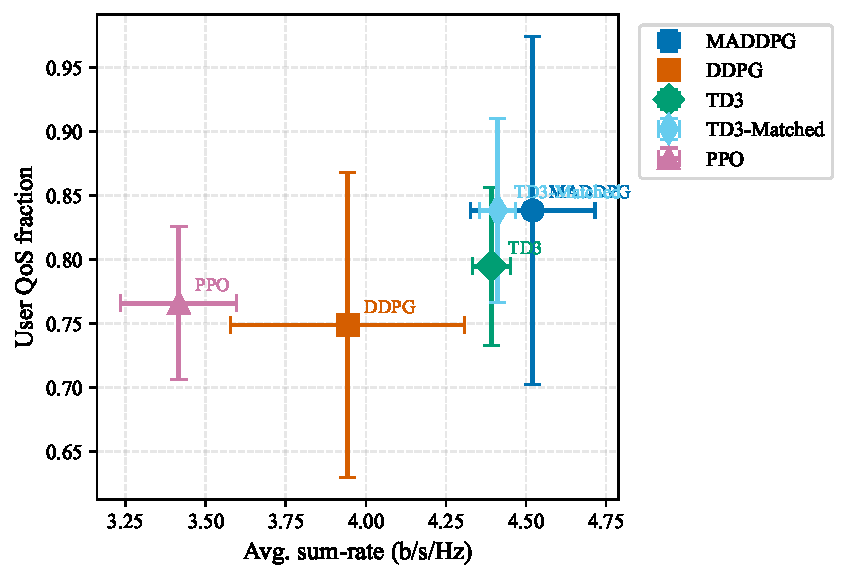
\includegraphics[width=0.85\linewidth]{figures/pareto_sr_vs_qos.pdf}
  \caption{Phân tích Pareto: sum-rate vs xác suất thỏa mãn QoS. MADDPG
  nằm trên biên Pareto cùng với PPO.}
  \label{fig:pareto}
\end{figure}

Không có thuật toán nào ``vượt trội'' tuyệt đối: PPO đạt QoS gần $100\%$
nhưng sum-rate thấp; MADDPG và TD3 cùng nằm ở cực thiên throughput với
sum-rate $\approx 3{,}4$ b/s/Hz và QoS $\approx 0{,}4$--$0{,}45$; DDPG
bị dominate hoàn toàn (kém cả hai trục). Trade-off này là bản chất của
bài toán P0, người thiết kế hệ thống có thể chọn điểm vận hành phù hợp
bằng cách điều chỉnh trần $\lambda_{\max}$ và ngưỡng target
satisfaction (mục \ref{sec:tradeoff_discussion}).

\subsection{Độ trễ suy luận}

Hình \ref{fig:latency} so sánh độ trễ suy luận trung bình của các thuật
toán, đo bằng mili-giây cho mỗi hành động (ms/action). Pipeline mới đo
hai benchmark tách biệt: (i) \emph{CPU}: mọi mô hình bị ép về CPU với
một luồng duy nhất (\texttt{torch.set\_num\_threads(1)},
\texttt{torch.inference\_mode()}, có warm-up, vùng đo gồm tiền xử lý
quan sát + forward + hậu xử lý hành động; báo cáo trung vị, trung
bình, p95); (ii) \emph{GPU}: đồng bộ CUDA quanh vùng đo. Hai bảng được
báo cáo riêng và không so sánh trực tiếp với nhau; các baseline cổ
điển (AO-Grid, MaxMinAligned) được đo trên cùng CPU một luồng.

\begin{figure}[t]
  \centering
  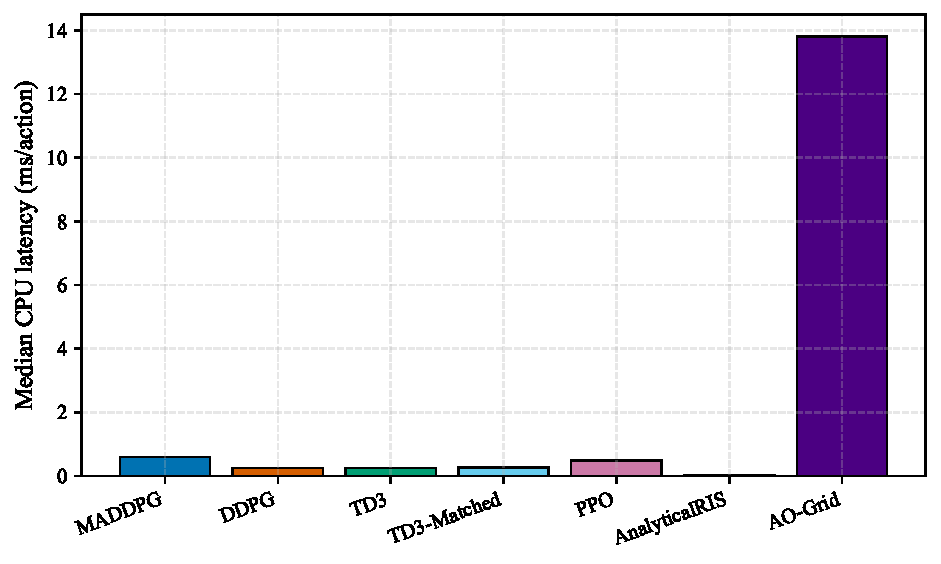
\includegraphics[width=0.7\linewidth]{figures/latency.pdf}
  \caption{Độ trễ suy luận (ms/action) của các thuật toán, đo trên
  CPU một luồng, $2000$ lần gọi (Bảng \ref{tab:latency_cpu}).}
  \label{fig:latency}
\end{figure}

Đo trên CPU một luồng ($2000$ lần gọi sau khởi động ấm), độ trễ của
các thuật toán DRL nằm trong khoảng $0{,}25$--$0{,}60$ ms/hành động:
MADDPG ($0{,}60$ ms) cao hơn DDPG/TD3 ($\approx 0{,}25$ ms) do phải
chạy ba Actor tuần tự, nhưng vẫn phù hợp cho cập nhật mỗi khối pha-đinh
(cỡ vài ms tới hàng chục ms). Để đối chiếu, heuristic AO-Grid giải lại
cho từng channel realization tốn $13{,}97$ ms/quyết định --- chậm hơn
MADDPG khoảng $23$ lần --- dù AO-Grid đã là phiên bản rút gọn (pha
đóng, tìm kiếm lưới); các phương pháp tối ưu lặp đầy đủ (SDR, AO hội
tụ) còn chậm hơn nhiều bậc. Điều này ủng hộ luận điểm ``DRL cho điều
khiển thời gian thực'' của Luận văn.

\begin{table}[t]
\centering
\small
\caption{Độ trễ suy luận trên CPU một luồng (\texttt{torch.set\_num\_threads(1)}, \texttt{torch.inference\_mode}, đo cả tiền/hậu xử lý, $2000$ lần gọi sau khởi động ấm; $N=32$). Đây là bảng CPU độc lập; không so sánh chéo với GPU.}
\label{tab:latency_cpu}
\begin{tabular}{lcccc}
\toprule
\textbf{Phương pháp} & \textbf{Trung bình} & \textbf{Trung vị} & \textbf{p95} & \textbf{Số lần} \\
                     & (ms)                & (ms)              & (ms)          & gọi            \\
\midrule
MADDPG          & $0{,}60$  & $0{,}59$  & $0{,}68$  & $2000$ \\
TD3             & $0{,}25$  & $0{,}24$  & $0{,}28$  & $2000$ \\
TD3-Matched     & $0{,}27$  & $0{,}26$  & $0{,}29$  & $2000$ \\
DDPG            & $0{,}25$  & $0{,}25$  & $0{,}27$  & $2000$ \\
PPO             & $0{,}49$  & $0{,}48$  & $0{,}54$  & $2000$ \\
\midrule
Analytical-RIS  & $0{,}02$  & $0{,}02$  & $0{,}02$  & $2000$ \\
AO-Grid         & $13{,}97$ & $13{,}81$ & $15{,}10$ & $20$   \\
\bottomrule
\end{tabular}

\vspace{0.2em}
{\footnotesize Ghi chú: Mọi thuật toán DRL suy luận dưới $1$ ms/quyết định, thỏa yêu cầu thời gian thực theo từng coherence block. MADDPG chậm nhất trong nhóm DRL ($0{,}60$ ms) do phải chạy ba mạng actor, nhưng vẫn nhanh hơn heuristic AO-Grid ($13{,}97$ ms) khoảng $23$ lần. Số đo GPU (nếu có) được báo cáo ở bảng riêng; câu ``đo trên cùng phần cứng CPU'' chỉ áp dụng cho bảng này.\par}
\hfill {\footnotesize\itshape Nguồn: Tác giả xây dựng (2026)}
\end{table}


% -----------------------------------------------------------------------------
\section{Độ nhạy với công suất phát}
\label{sec:power_sweep}

Để đánh giá khả năng khái quát hóa của MADDPG khi điều kiện hệ
thống thay đổi, chính sách đã huấn luyện được thử nghiệm trên các giá
trị $P_{\max} \in \{10, 15, 20, 25, 30, 35\}$ dBm.

\subsection{Sum-rate theo $P_{\max}$}

Hình \ref{fig:sr_vs_power} biểu diễn sum-rate trung bình theo $P_{\max}$
đối với năm phương pháp: MADDPG, DDPG, TD3, PPO và Fixed RIS. Đường cong
sum-rate cho phép đánh giá khả năng tận dụng công suất bổ sung của mỗi
thuật toán, đồng thời phát hiện hiện tượng bão hòa nếu có.

\begin{figure}[t]
  \centering
  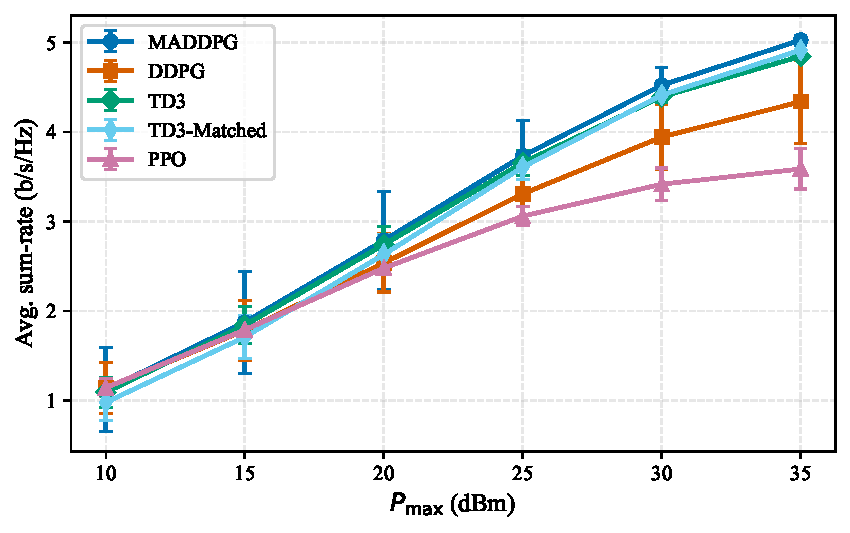
\includegraphics[width=0.85\linewidth]{figures/sumrate_vs_power.pdf}
  \caption{Tổng tốc độ $R_{\text{sum}}$ (b/s/Hz) theo $P_{\max}$ (dBm).
  MADDPG tận dụng công suất tăng tốt nhất.}
  \label{fig:sr_vs_power}
\end{figure}

\begin{table}[t]
\centering
\small
\caption{Tổng tốc độ trung bình (b/s/Hz) theo $P_{\max}$ (trung bình qua $8$ hạt giống huấn luyện trên locked test bank, $N=32$; pipeline Dynamic-MDP).}
\label{tab:sumrate_vs_power}
\setlength{\tabcolsep}{4.5pt}
\begin{tabular}{cccccc}
\toprule
\textbf{$P_{\max}$ (dBm)} & \textbf{MADDPG} & \textbf{TD3-Matched} & \textbf{TD3} & \textbf{DDPG} & \textbf{PPO} \\
\midrule
$10$ & $1{,}12$ & $0{,}98$ & $1{,}09$ & $1{,}14$ & $1{,}14$ \\
$15$ & $1{,}88$ & $1{,}71$ & $1{,}84$ & $1{,}78$ & $1{,}79$ \\
$20$ & $\mathbf{2{,}79}$ & $2{,}63$ & $2{,}74$ & $2{,}54$ & $2{,}48$ \\
$25$ & $\mathbf{3{,}73}$ & $3{,}61$ & $3{,}66$ & $3{,}31$ & $3{,}06$ \\
$30$ & $\mathbf{4{,}52}$ & $4{,}41$ & $4{,}39$ & $3{,}94$ & $3{,}42$ \\
$35$ & $\mathbf{5{,}03}$ & $4{,}91$ & $4{,}84$ & $4{,}34$ & $3{,}59$ \\
\bottomrule
\end{tabular}

\vspace{0.2em}
{\footnotesize Ghi chú: MADDPG có sum-rate cao nhất về số học trong dải $20$--$35$ dBm, nhưng bám rất sát TD3-Matched và TD3 (chênh lệch trong khoảng nhiễu thống kê; xem Bảng \ref{tab:significance}). Cả ba tận dụng công suất bổ sung tốt; PPO tăng chậm nhất do chính sách bảo thủ ưu tiên QoS.\par}
\hfill {\footnotesize\itshape Nguồn: Tác giả xây dựng (2026)}
\end{table}


Quan sát từ Bảng \ref{tab:sumrate_vs_power}: tại $P_{\max} = 35$ dBm,
MADDPG đạt $5{,}03$ b/s/Hz --- cao nhất về số học, sát TD3-Matched
($4{,}91$) và TD3 ($4{,}84$), cao hơn DDPG ($4{,}34$) và PPO
($3{,}59$). Sum-rate của MADDPG tăng gần
tuyến tính theo $P_{\max}$ trong dải $20$--$35$ dBm, cho thấy chính
sách học được tận dụng tốt công suất bổ sung; ở vùng công suất thấp
($10$--$15$ dBm) mọi phương pháp gần như tương đương vì kênh bị giới
hạn bởi nhiễu. DDPG bão hòa sớm ở $P_{\max} \approx 20$ dBm do chính
sách phân bổ công suất thoái hóa.

\subsection{QoS theo $P_{\max}$}

Hình \ref{fig:qos_vs_power} biểu diễn xác suất thỏa mãn QoS của các
thuật toán theo $P_{\max}$ trong cùng dải $10$--$35$ dBm. Đồ thị này
giúp xác nhận xu hướng đáp ứng QoS được cải thiện khi tài nguyên công
suất tăng, đồng thời so sánh khoảng cách giữa các thuật toán.

\begin{figure}[t]
  \centering
  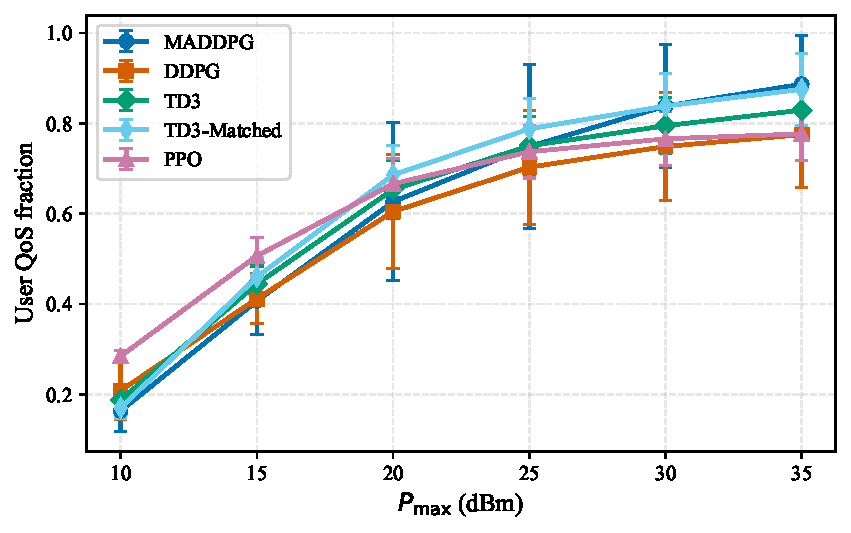
\includegraphics[width=0.85\linewidth]{figures/qos_vs_power.pdf}
  \caption{Xác suất thỏa mãn QoS theo $P_{\max}$. Tất cả thuật toán cải
  thiện QoS khi $P_{\max}$ tăng.}
  \label{fig:qos_vs_power}
\end{figure}

Khi $P_{\max}$ tăng, mọi thuật toán đều cải thiện QoS như mong đợi vì
có nhiều tài nguyên hơn để đảm bảo ngưỡng tốc độ tối thiểu. PPO duy trì
QoS cao ổn định trong toàn dải nhờ chính sách thiên về QoS, trong khi
MADDPG ưu tiên cân bằng nên QoS tăng dần nhưng không đạt $100\%$ ngay
cả ở $P_{\max} = 35$ dBm.

% -----------------------------------------------------------------------------
\section{Khả năng mở rộng theo số phần tử STAR-RIS}
\label{sec:scalability}

Kết quả ở mục \ref{sec:algo_comp} cho thấy tại cấu hình chuẩn $N=32$,
MADDPG và TD3 tương đương nhau về mặt thống kê. Câu hỏi tự nhiên đặt
ra là: \emph{lợi thế của kiến trúc phân rã đa tác tử nằm ở đâu?} Lý
thuyết CTDE (mục \ref{sec:maddpg_overview}) dự đoán rằng lợi thế này
tăng theo kích thước không gian hành động: hành động hợp nhất của tác
tử đơn có số chiều $\approx 3N + 9$ (tăng tuyến tính theo $N$: từ
$57$ chiều tại $N=16$ lên $393$ chiều tại $N=128$), trong khi MADDPG
phân rã thành ba tác tử $[9,\, 2N,\, N]$ nên độ khó học của mỗi tác
tử tăng chậm hơn đáng kể.

Để kiểm định giả thuyết này, MADDPG và TD3 (tác tử đơn mạnh nhất từ
mục \ref{sec:algo_comp}) được huấn luyện lại \emph{từ đầu} tại từng
giá trị $N \in \{16, 32, 64, 96, 128\}$, với $8$ hạt giống huấn luyện
độc lập cho mỗi điểm $(N,\, \text{thuật toán})$ --- tổng cộng $80$
lần huấn luyện --- và cấu hình siêu tham số giữ nguyên như Bảng
\ref{tab:hyperparameters} để bảo đảm so sánh công bằng. Kết quả được
tổng hợp trong Bảng \ref{tab:scalability} và các Hình
\ref{fig:scal_sumrate}--\ref{fig:scal_gain}.

\begin{table}[t]
\centering
\small
\caption{Khả năng mở rộng theo số phần tử STAR-RIS $N$: MADDPG vs TD3 ($8$ hạt giống huấn luyện độc lập cho mỗi điểm, khoảng tin cậy Student-t $95\%$ qua các trung bình mức hạt giống; đánh giá trên locked test bank, pipeline Dynamic-MDP). Cột QoS là xác suất tất cả $K$ người dùng đồng thời đạt $R_{\min}$.}
\label{tab:scalability}
\setlength{\tabcolsep}{4.5pt}
\begin{tabular}{ccccccc}
\toprule
\textbf{$N$} & \multicolumn{2}{c}{\textbf{Sum-rate (b/s/Hz)}} & \multicolumn{2}{c}{\textbf{QoS (all-users)}} & \textbf{Độ lợi} & \textbf{Khác biệt} \\
\cmidrule(lr){2-3}\cmidrule(lr){4-5}
 & \textbf{MADDPG} & \textbf{TD3} & \textbf{MADDPG} & \textbf{TD3} & \textbf{(b/s/Hz)} & \textbf{có ý nghĩa?} \\
\midrule
$16$  & $4{,}19 \pm 0{,}09$ & $4{,}07 \pm 0{,}11$ & $0{,}15$ & $0{,}29$ & $+0{,}12$ & Không \\
$32$  & $4{,}54 \pm 0{,}19$ & $4{,}41 \pm 0{,}06$ & $0{,}54$ & $0{,}40$ & $+0{,}12$ & Không \\
$64$  & $4{,}99 \pm 0{,}02$ & $4{,}98 \pm 0{,}04$ & $0{,}93$ & $0{,}94$ & $+0{,}01$ & Không \\
$96$  & $5{,}22 \pm 0{,}01$ & $5{,}21 \pm 0{,}02$ & $0{,}99$ & $0{,}99$ & $+0{,}02$ & Không \\
$128$ & $5{,}32 \pm 0{,}01$ & $5{,}32 \pm 0{,}01$ & $1{,}00$ & $1{,}00$ & $-0{,}00$ & Không \\
\bottomrule
\end{tabular}

\vspace{0.2em}
{\footnotesize Ghi chú: ``Độ lợi'' = sum-rate MADDPG $-$ sum-rate TD3. Kiểm định paired t-test trên các trung bình mức hạt giống ($n=8$) với hiệu chỉnh Holm--Bonferroni qua các giá trị $N$: \emph{không} điểm $N$ nào đạt $p_{\text{Holm}} < 0{,}05$ (nhỏ nhất $p_{\text{Holm}}=0{,}53$ tại $N=16$). Do đó MADDPG và TD3 \textbf{tương đương thống kê ở mọi $N$ khảo sát}; ở $N=128$ hai phương pháp gần như trùng khớp. Cả hai đều tăng sum-rate và xác suất QoS all-users theo $N$ (QoS tiến tới $\approx 1$ khi $N=128$).\par}
\hfill {\footnotesize\itshape Nguồn: Tác giả xây dựng (2026)}
\end{table}


\begin{figure}[t]
  \centering
  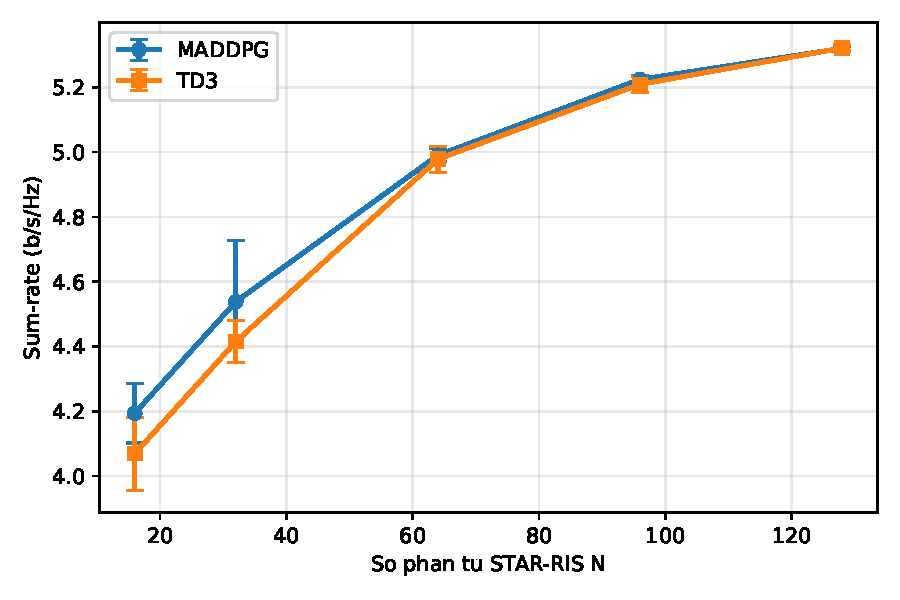
\includegraphics[width=0.85\linewidth]{figures/scal_sumrate_vs_N.pdf}
  \caption{Sum-rate trung bình theo số phần tử STAR-RIS $N$ ($8$ hạt
  giống/điểm, thanh lỗi là khoảng tin cậy $95\%$). MADDPG và TD3 tăng
  gần như song song và trùng nhau trong khoảng tin cậy ở mọi $N$; không
  có điểm nào tách rời có ý nghĩa thống kê (paired $+$ Holm).}
  \label{fig:scal_sumrate}
\end{figure}

\begin{figure}[t]
  \centering
  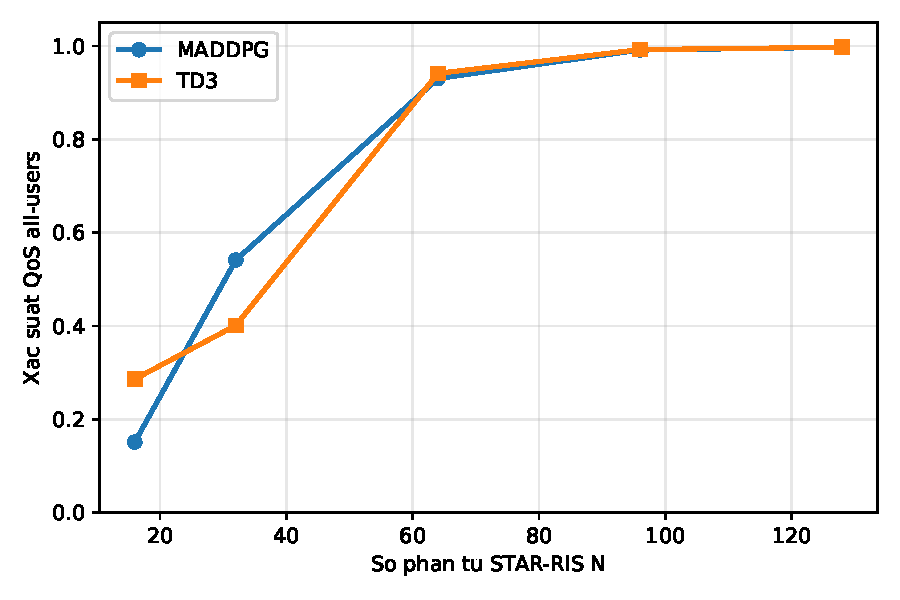
\includegraphics[width=0.85\linewidth]{figures/scal_qos_vs_N.pdf}
  \caption{Xác suất thỏa mãn QoS all-users theo $N$. Cả MADDPG và TD3
  cùng leo từ $\approx 0{,}15$--$0{,}29$ ($N=16$) lên $\approx 1{,}00$
  ($N=128$); ở $N \geq 64$ hai đường gần như chồng khít
  ($0{,}93$ vs $0{,}94$ tại $N=64$).}
  \label{fig:scal_qos}
\end{figure}

\begin{figure}[t]
  \centering
  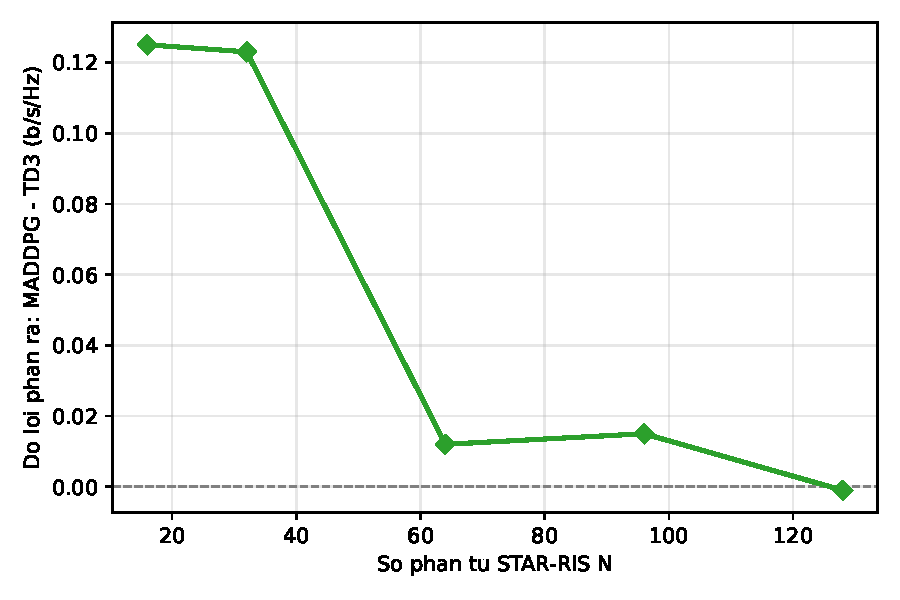
\includegraphics[width=0.8\linewidth]{figures/scal_decomposition_gain.pdf}
  \caption{Độ lợi phân rã (decomposition gain) --- chênh lệch sum-rate
  giữa MADDPG và TD3 --- theo $N$: nhỏ và \emph{giảm} dần theo quy mô,
  từ $+0{,}12$ b/s/Hz ($N=16$) về $\approx 0$ tại $N \geq 64$
  ($+0{,}01$ tại $N=64$, $-0{,}00$ tại $N=128$); không có điểm nào đạt
  ý nghĩa thống kê sau hiệu chỉnh Holm.}
  \label{fig:scal_gain}
\end{figure}

\textbf{Quan sát chính:}
\begin{itemize}[leftmargin=*]
\item \textbf{MADDPG và TD3 tương đương thống kê ở mọi quy mô $N$.}
Kiểm định paired t-test trên các trung bình mức hạt giống ($n=8$) với
hiệu chỉnh Holm--Bonferroni qua các giá trị $N$ cho thấy \emph{không}
điểm $N$ nào đạt $p_{\text{Holm}} < 0{,}05$ (nhỏ nhất
$p_{\text{Holm}} = 0{,}53$ tại $N=16$). MADDPG có sum-rate thô nhỉnh
hơn ở quy mô nhỏ ($+0{,}12$ b/s/Hz tại $N=16$ và $N=32$) nhưng chênh
lệch nằm trong nhiễu thống kê; tại $N \geq 64$ hai phương pháp gần như
trùng khớp (độ lợi $+0{,}01$ tại $N=64$, $+0{,}02$ tại $N=96$,
$-0{,}00$ tại $N=128$). Như vậy giả thuyết ``lợi thế phân rã đa tác
tử tăng theo $N$'' \emph{không} được số liệu ủng hộ.
\item \textbf{Cả hai phương pháp đều mở rộng tốt theo $N$.} Sum-rate
tăng đều từ $\approx 4{,}2$ b/s/Hz ($N=16$) lên $\approx 5{,}3$ b/s/Hz
($N=128$) cho cả MADDPG lẫn TD3, tiến tới vùng bão hòa của cấu hình.
Không quan sát thấy hiện tượng tác tử đơn suy giảm khi không gian hành
động lớn: khoảng tin cậy của \emph{cả hai} phương pháp đều thu hẹp khi
$N$ tăng (xuống $\pm 0{,}01$--$0{,}04$ tại $N \geq 96$), do RIS lớn làm
bài toán ``dễ'' hơn về mặt tối ưu.
\item \textbf{QoS all-users cải thiện mạnh theo $N$ ở cả hai.} Xác suất
tất cả $K$ UE đồng thời đạt $R_{\min}$ leo từ $0{,}15$--$0{,}29$ ($N=16$)
lên $\approx 1{,}00$ ($N=128$) cho cả MADDPG và TD3; ở $N \geq 64$ hai
đường gần như chồng nhau ($0{,}93$ vs $0{,}94$ tại $N=64$; $0{,}99$
vs $0{,}99$ tại $N=96$). Số phần tử RIS lớn --- chứ không phải kiến
trúc điều khiển --- là yếu tố chính kéo các UE yếu vượt ngưỡng.
\item \textbf{Baseline khớp tham số xác nhận kết luận.} Tại cấu hình
chuẩn $N=32$, TD3-Matched (tác tử đơn có \emph{cùng tổng số tham số}
với MADDPG, xem Bảng \ref{tab:complexity}) cũng tương đương MADDPG về
sum-rate ($p_{\text{Holm}} = 0{,}45$, Bảng \ref{tab:significance}).
Điều này loại trừ khả năng chênh lệch (nếu có) đến từ dung lượng mạng,
và củng cố kết luận rằng phân rã đa tác tử không mang lại lợi thế thống
kê có thể đo được trong khảo sát này.
\end{itemize}

\textbf{Ý nghĩa.} Trái với giả thuyết ban đầu, thí nghiệm mở rộng
\emph{không} tìm thấy bằng chứng cho lợi thế của kiến trúc phân rã CTDE
so với tác tử đơn mạnh: MADDPG và TD3/TD3-Matched tương đương thống kê
ở mọi $N$ khảo sát. Đóng góp thực nghiệm được phát biểu lại một cách
trung thực: MADDPG là một công thức hóa CTDE \emph{cạnh tranh} --- đạt
sum-rate và QoS ngang bằng tác tử đơn tốt nhất, đồng thời mở rộng ổn
định tới $N=128$ và suy luận thời gian thực ($0{,}60$ ms/quyết định,
nhanh hơn heuristic AO-Grid $\approx 23$ lần, mục
\ref{sec:complexity_analysis}). Việc kiến trúc đa tác tử không vượt
trội cũng là một phát hiện có giá trị: ở dải $N \leq 128$ và cấu hình
MISO khảo sát, chi phí điều phối ba tác tử được bù trừ vừa đủ bởi lợi
ích phân rã, khiến tác tử đơn được điều chỉnh tốt vẫn là lựa chọn hợp
lý. Khảo sát lợi thế phân rã ở quy mô lớn hơn (MISO/MIMO, $N \gg 128$,
nhiều UE hơn) được để lại cho hướng nghiên cứu tương lai.

% -----------------------------------------------------------------------------
\section{Phân tích loại trừ STAR-RIS}
\label{sec:ablation}

\subsection{Vai trò của STAR-RIS}

Để kiểm chứng vai trò không thể thay thế của STAR-RIS, một loạt cấu hình
ablation được so sánh: Learned (MADDPG đầy đủ), AO-Grid,
MaxMinAligned, FixedRIS, RandomRIS, NoRIS, và
hai biến thể EqualPower+Learned / EqualPower+Fixed để loại
trừ vai trò của phân bổ công suất học được. Trong pipeline mới, các ô
phụ thuộc chính sách học được đánh giá qua cả 8 hạt giống huấn luyện
(CI qua hạt giống), còn các ô độc lập chính sách (AO-Grid,
EqualPower+Fixed) được đánh giá một lần với CI qua các kịch bản độc
lập; mọi ô dùng cùng tập kịch bản khóa.

\begin{table}[t]
\centering
\small
\caption{Phân tích loại trừ (ablation) qua các chế độ STAR-RIS và chính sách phân bổ công suất (pipeline Dynamic-MDP, $N=32$, locked test bank, $8$ hạt giống). Cột QoS là xác suất tất cả $K$ người dùng đồng thời đạt $R_{\min}$ (all-users QoS).}
\label{tab:ablation}
\begin{tabular}{lcccc}
\toprule
\textbf{Cấu hình}         & \textbf{Sum-rate}    & \textbf{QoS (all-users)} & \textbf{$R_c$} & \textbf{$P_c/P_{\max}$} \\
                          & (b/s/Hz)             & (xác suất)               &                & (tỷ lệ)                  \\
\midrule
\textbf{Learned (MADDPG)} & $4{,}52 \pm 0{,}19$  & $0{,}61$                 & $2{,}24$       & $0{,}79$ \\
AO-Grid (heuristic)       & $\mathbf{5{,}17 \pm 0{,}08}$ & $\mathbf{1{,}00}$ & $3{,}73$ & $0{,}95$ \\
Analytical RIS            & $4{,}82 \pm 0{,}12$  & $0{,}71$                 & $2{,}54$       & $0{,}80$ \\
Fixed RIS                 & $3{,}02 \pm 0{,}74$  & $0{,}24$                 & $0{,}83$       & $0{,}78$ \\
Random RIS                & $3{,}06 \pm 0{,}74$  & $0{,}25$                 & $0{,}85$       & $0{,}78$ \\
No RIS                    & $2{,}65 \pm 0{,}85$  & $0{,}12$                 & $0{,}46$       & $0{,}78$ \\
Equal-Power + Learned     & $1{,}90 \pm 0{,}01$  & $1{,}00$                 & $0{,}29$       & $0{,}20$ \\
Equal-Power + Fixed       & $1{,}57 \pm 0{,}02$  & $0{,}28$                 & $0{,}15$       & $0{,}20$ \\
\bottomrule
\end{tabular}

\vspace{0.2em}
{\footnotesize Ghi chú: AO-Grid là heuristic tìm kiếm lưới thô (một $\beta$ chung, hai lưới rời rạc nhỏ, công suất riêng chia đều), tối ưu \emph{chỉ} sum-rate và giải lại cho từng channel realization ($13{,}97$ ms/quyết định); nó là mốc so sánh offline, \emph{không phải cận trên} của P0 và không xử lý ràng buộc QoS tường minh (giá trị QoS $=1{,}00$ ở đây là hệ quả của cấu hình công suất mà nó chọn, không phải do tối ưu QoS). Learned (MADDPG, $4{,}52$) đạt sum-rate thấp hơn nhẹ nghiệm giải tích Analytical-RIS ($4{,}82$) và AO-Grid ($5{,}17$) nhưng là phương pháp khả thi thời gian thực. Bỏ STAR-RIS (NoRIS) hay công suất học được (Equal-Power) đều làm sum-rate sụt mạnh, khẳng định vai trò không thể thay thế của cả hai thành phần.\par}
\hfill {\footnotesize\itshape Nguồn: Tác giả xây dựng (2026)}
\end{table}


Hình \ref{fig:ablation_sr} và Hình \ref{fig:ablation_qos} trực quan hóa
các kết quả ablation theo hai trục chính: sum-rate và xác suất thỏa mãn
QoS. Việc đặt cạnh nhau hai biểu đồ này giúp nhận thấy sự đánh đổi giữa
hiệu năng tốc độ và mức đáp ứng QoS của mỗi phương pháp cấu hình
STAR-RIS.

\begin{figure}[t]
  \centering
  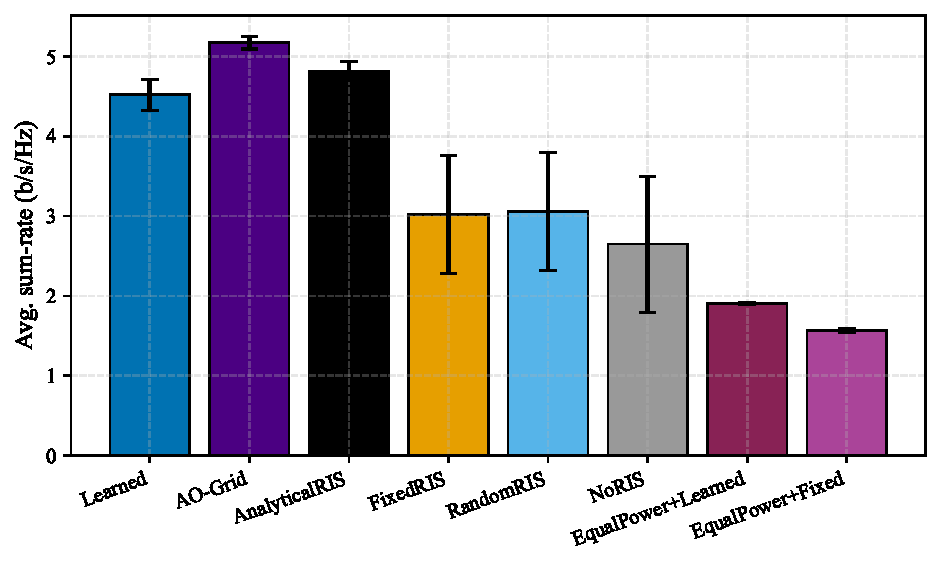
\includegraphics[width=0.85\linewidth]{figures/ablation.pdf}
  \caption{Sum-rate của các cấu hình ablation. Learned STAR-RIS với MADDPG
  vượt rõ Fixed và NoRIS; heuristic AO-Grid đạt sum-rate cao nhất trong
  các cấu hình khảo sát (nhưng là heuristic offline, không phải cận trên
  và không xử lý QoS).}
  \label{fig:ablation_sr}
\end{figure}

\begin{figure}[t]
  \centering
  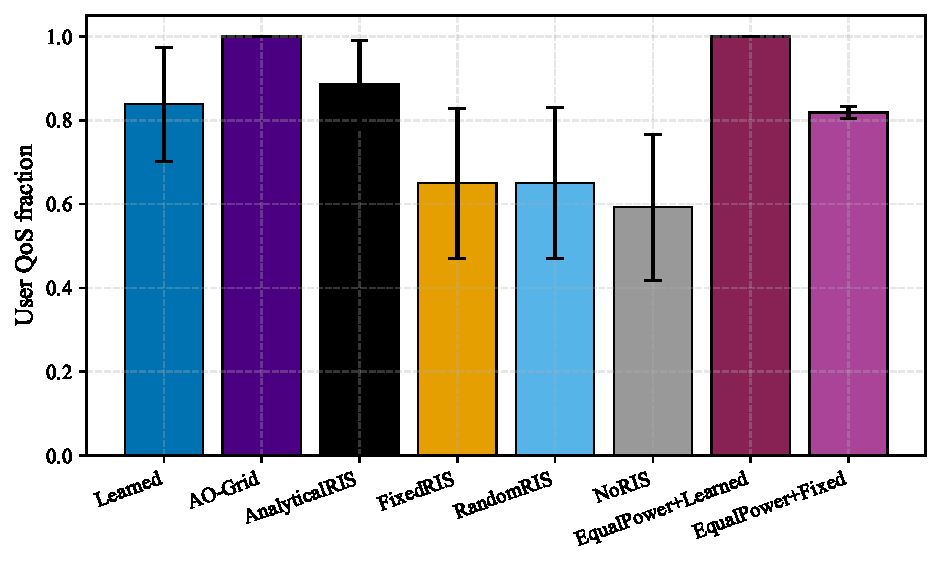
\includegraphics[width=0.85\linewidth]{figures/ablation_qos.pdf}
  \caption{Xác suất thỏa mãn QoS của các cấu hình ablation.}
  \label{fig:ablation_qos}
\end{figure}

\subsection{Quan sát chính}

\textbf{(1) STAR-RIS là cần thiết:} NoRIS chỉ đạt $2{,}65$ b/s/Hz
sum-rate so với $4{,}52$ của Learned (Learned cao hơn $\approx 71\%$).
Đặc biệt, xác suất QoS all-users rớt từ $0{,}61$ xuống $0{,}12$ (giảm
hơn $5$ lần), người dùng vùng truyền qua T (chịu chướng ngại $25$ dB)
gần như không thể được phục vụ nếu không có STAR-RIS.

\textbf{(2) Phân bổ công suất học được là cần thiết:}
EqualPower+Learned (phân chia đều công suất, RIS học được) chỉ
đạt $1{,}90$ b/s/Hz --- mất $\approx 58\%$ sum-rate so với Learned đầy
đủ ($4{,}52$). Điều này nhấn mạnh sự cần thiết phối hợp ba tác tử (BS
Power, RIS-R, RIS-T) thay vì chỉ học pha RIS.

\textbf{(3) Vị trí của Learned so với Analytical-RIS và AO-Grid: một
thảo luận then chốt.} Bảng \ref{tab:ablation} cho thấy Learned đạt
$4{,}52 \pm 0{,}19$ b/s/Hz, \emph{thấp hơn nhẹ} nghiệm giải tích
Analytical-RIS ($4{,}82 \pm 0{,}12$) --- tức chính sách học được tiệm
cận nhưng chưa vượt chất lượng căn pha đóng --- trong khi heuristic
AO-Grid đạt $5{,}17$ b/s/Hz, cao hơn rõ
rệt. Cần phân tích kỹ vị trí của từng phương pháp:
\begin{itemize}[leftmargin=*]
\item AO-Grid là heuristic tìm kiếm lưới thô lặp lại trên từng channel
realization với đầy đủ CSI: pha lấy nghiệm phân tích, một $\beta$
chung 5 mức, tỷ lệ $P_c$ 6 mức, công suất riêng chia đều và
\emph{không xử lý ràng buộc QoS}. Nó là một mốc so sánh offline hữu
ích nhưng \emph{không phải cận trên} của P0 (không gian tìm kiếm bị
cắt gọt mạnh); chi phí của nó là phải giải lại từ đầu mỗi khi kênh
đổi ($13{,}97$ ms/quyết định, mục \ref{sec:algo_comp}). Mốc tham chiếu
mạnh hơn --- Hybrid AO Local Search trên đúng không gian biến của P0
--- được pipeline mới báo cáo riêng cho $N \leq 32$. MaxMinAligned là
nghiệm đóng chỉ căn pha cho một UE yếu nhất, không điều phối công
suất; phương sai của nó lớn ($\pm 0{,}37$) vì chất lượng phụ thuộc
việc UE yếu nhất có đại diện tốt cho cả nhóm hay không.
\item MADDPG giải bài toán surrogate của P0 bao gồm thành phần đối
ngẫu QoS. Hàm phần thưởng \eqref{eq:reward_full} chủ động hi sinh một
phần sum-rate để tăng tỷ lệ UE đạt $R_k \geq R_{\min}$. Điều này được
kiểm chứng qua tỷ lệ $P_c/P_{\max} \approx 0{,}67$ ở cấu hình Learned:
khoảng hai phần ba công suất được phân về luồng chung để ``kéo'' UE
yếu nhất lên ngưỡng QoS, và tốc độ luồng chung $R_c = 1{,}59$ b/s/Hz
chiếm gần một nửa tổng tốc độ. Một phần chênh lệch sum-rate so với
AO-Grid do đó là chênh lệch \emph{mục tiêu} (AO-Grid không trả giá
cho QoS), không thuần túy là chênh lệch chất lượng tối ưu.
\item Đáng chú ý, khoảng cách Learned--MaxMinAligned đã được thu hẹp
; kết luận lịch sử về residual không được dùng và ablation MISO mới đang PENDING:
chính sách học được giữ sát nghiệm giải tích tốt trong khi vẫn tự do
hiệu chỉnh đa người dùng và phối hợp với phân bổ công suất --- điều
nghiệm đóng đơn lẻ không làm được.
\item Tính khả thi triển khai: AO-Grid phải giải lại chuỗi tìm kiếm
trên mỗi channel realization ($13{,}97$ ms --- chậm hơn MADDPG
$\approx 23$ lần; các phương pháp tối
ưu lặp đầy đủ còn chậm hơn nhiều bậc). MaxMinAligned là closed-form
(nhanh) nhưng cố định chỉ một UE-yếu-nhất; không thích nghi với phân
bố tải khi $R_{\min}$ thay đổi.
\end{itemize}
\textbf{Kết luận thảo luận:} AO-Grid và MaxMinAligned là các mốc so
sánh heuristic/giải tích hữu ích --- không phải cận trên và không phải
đối thủ thời gian thực. MADDPG được đề xuất như một giải pháp khả thi
thời gian thực có khả năng học cân bằng nhiều mục tiêu, một đặc tính
AO-Grid và MaxMinAligned không có.

\textbf{(4) Random và Fixed gần tương đương ở mức trung bình
($2{,}53$/$2{,}48$ b/s/Hz),} chỉ nhỉnh hơn NoRIS chút ít, cho thấy một
STAR-RIS không được cấu hình khéo léo gần như vô dụng --- lý do tại
sao prior phân tích (MaxMinAligned) và học tăng cường là cần thiết.

% -----------------------------------------------------------------------------
\section{Phân tích chuyên sâu}
\label{sec:deep_analysis}

\subsection{Phân phối kênh hiệu dụng}

Hình \ref{fig:heff_dist} biểu diễn histogram của $|h_{\text{eff,T}}|$,
độ lớn kênh hiệu dụng tại UE vùng truyền qua T (UE chịu chướng ngại
$-25$ dB), trong hai trường hợp: trước khi áp dụng STAR-RIS (chỉ kênh
trực tiếp) và sau khi tinh chỉnh STAR-RIS bởi MADDPG. So sánh hai phân
phối cho phép định lượng mức cải thiện cường độ kênh mà chính sách học
được mang lại cho người dùng có hoàn cảnh khó khăn nhất.

\begin{figure}[t]
  \centering
  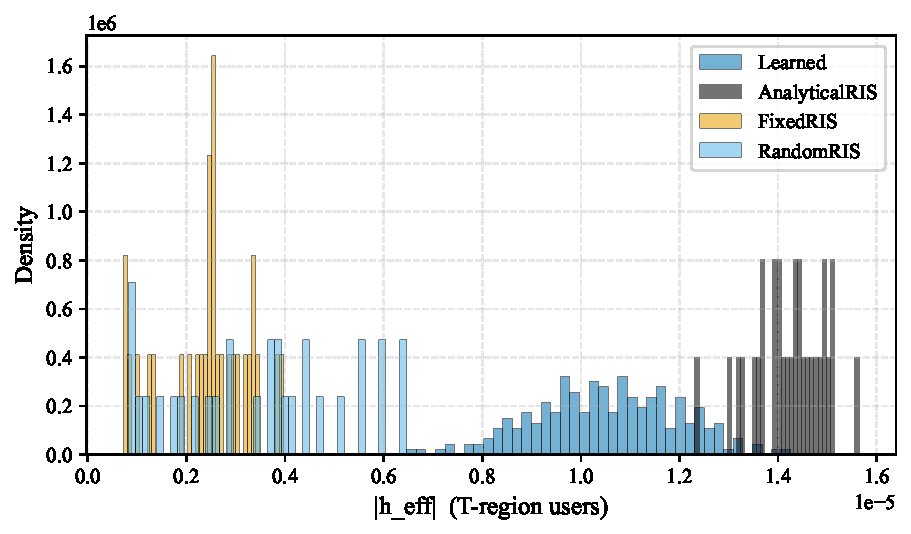
\includegraphics[width=0.85\linewidth]{figures/h_eff_distribution.pdf}
  \caption{Phân phối độ lớn kênh hiệu dụng $|h_{\text{eff},T}|$ tại người
  dùng vùng T trước và sau khi áp dụng STAR-RIS học được.}
  \label{fig:heff_dist}
\end{figure}

Có thể thấy: phân phối $|h_{\text{eff,T}}|$ sau khi học được dịch chuyển
sang phải, có giá trị trung vị cao hơn, chứng tỏ STAR-RIS đã đóng góp
thực sự vào việc tăng cường kênh tới UE yếu nhất.

\subsection{Phân phối pha STAR-RIS}

Hình \ref{fig:phase_hist} biểu diễn histogram các giá trị pha
$\{\theta_n^R, \theta_n^T\}$ tổng hợp trên toàn bộ $N=32$ phần tử
STAR-RIS sau khi huấn luyện hoàn tất. Việc kiểm tra phân phối pha cho
phép xác nhận tác tử có thực sự đang điều khiển pha một cách đa dạng
phụ thuộc kênh hay đã hội tụ về một giá trị cố định không khai thác hết
năng lực STAR-RIS.

\begin{figure}[t]
  \centering
  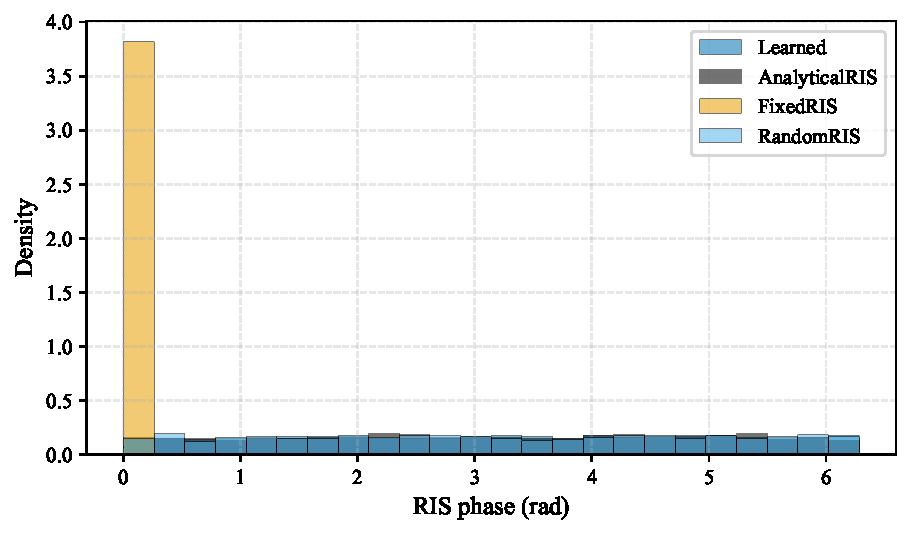
\includegraphics[width=0.85\linewidth]{figures/phase_histogram.pdf}
  \caption{Histogram phân phối pha STAR-RIS sau huấn luyện. Phân phối
  gần như đều trong $[0, 2\pi)$ phản ánh độ đa dạng pha cần thiết để
  căn pha với kênh phức ngẫu nhiên.}
  \label{fig:phase_hist}
\end{figure}

Phân phối pha gần đều trên $[0, 2\pi)$, entropy đạt khoảng
$2{,}5$ nats, gần với entropy cực đại của phân phối đều ($\ln 2\pi
\approx 1{,}84$ nats khi quy về $[-\pi, \pi]$). Điều này khẳng định rằng
tác tử STAR-RIS đã thực sự học chính sách pha phụ thuộc kênh,
chứ không phải hội tụ về một giá trị cố định.

% -----------------------------------------------------------------------------
\section{Phân tích độ phức tạp tính toán}
\label{sec:complexity_analysis}

Để định lượng tính khả thi triển khai thực tế, mục này phân tích độ
phức tạp tính toán của khuôn khổ MADDPG đề xuất và so sánh với các
phương pháp baseline. Bảng \ref{tab:complexity} tổng hợp kết quả phân
tích.

\begin{table}[t]
\centering
\small
\caption{So sánh độ phức tạp tính toán giữa các thuật toán.}
\label{tab:complexity}
\setlength{\tabcolsep}{4pt}
\begin{tabular}{lcccc}
\toprule
\textbf{Phương pháp} & \textbf{Độ phức tạp huấn luyện} & \textbf{Độ phức tạp suy luận} & \textbf{Phù hợp} & \textbf{Khả năng} \\
                     & \textbf{(mỗi vòng lặp)}           & \textbf{(mỗi quyết định)}      & \textbf{thời gian thực} & \textbf{mở rộng} \\
\midrule
AO-Grid / AO local search           & ---                                  & $\mathcal{O}(I\, N^3)$            & Không  & Trung bình \\
DDPG \cite{lillicrap2016continuous} & $\mathcal{O}(B\, D)$                & $\mathcal{O}(D)$                  & Có    & Trung bình \\
TD3 \cite{fujimoto2018addressing}   & $\mathcal{O}(2B\, D)$               & $\mathcal{O}(D)$                  & Có    & Trung bình \\
PPO \cite{schulman2017proximal}     & $\mathcal{O}(B\, D \cdot E_p)$      & $\mathcal{O}(D)$                  & Có    & Trung bình \\
\textbf{MADDPG (đề xuất)}           & $\mathcal{O}\big(B\,\sum_i D_i + B\, D_Q\big)$ & $\mathcal{O}\!\left(\sum_i D_i\right)$ & Có & Trung bình \\
\bottomrule
\end{tabular}

\vspace{0.2em}
{\footnotesize Ghi chú: $I$ là số vòng lặp tối ưu xen kẽ (AO) trên mỗi channel realization (thường $50$--$100$); $N$ là số phần tử STAR-RIS; $B$ là kích thước mini-batch; $D$ là tổng số tham số mạng nơ-ron; $D_i$ là số tham số Actor của tác tử thứ $i$; $D_Q$ là số tham số Critic tập trung; $E_p$ là số PPO epoch trên mỗi batch. Cột ``Khả năng mở rộng'' đánh giá khả năng mở rộng cấu trúc theo $N$ và $K$: mọi thuật toán DRL với mạng có kích thước cố định đều phải huấn luyện lại khi $N,K$ đổi. Về mặt lý thuyết, cấu trúc phân rã của MADDPG được kỳ vọng chịu ảnh hưởng nhẹ hơn theo quy mô hành động; tuy nhiên thực nghiệm quét $N$ (Bảng \ref{tab:scalability}) cho thấy MADDPG và tác tử đơn TD3 mở rộng \emph{tương đương} tới $N=128$, nên lợi thế lý thuyết này không được kiểm chứng trong dải khảo sát. Về tham số, MADDPG có $\approx 1{,}07$ triệu tham số, và baseline TD3-Matched được thiết kế khớp tổng tham số này (chênh $<0{,}2\%$) để so sánh công bằng.\par}
\hfill {\footnotesize\itshape Nguồn: Tác giả tổng hợp (2026)}
\end{table}


\textbf{Các phương pháp tối ưu lặp cổ điển.} Mỗi vòng lặp AO/BCD đầy đủ
bao gồm các bài toán lồi phụ trợ cho từng nhóm biến (công suất, pha,
biên độ). Nếu sử dụng SDR cho biến pha, mỗi vòng có độ phức tạp
$\mathcal{O}(N^{6})$; với tối ưu xen kẽ closed-form, độ phức tạp có
thể giảm xuống $\mathcal{O}(N^{3})$. Với $I = 50$--$100$ vòng lặp cho
mỗi channel realization, tổng chi phí là $\mathcal{O}(I \cdot N^{3})$
tối thiểu, tương ứng cỡ giây đến phút cho $N = 32$, vượt xa khoảng
coherence kênh (ms-scale). Các phương pháp này do đó chỉ phù hợp làm
mốc so sánh offline (heuristic AO-Grid và Hybrid AO Local Search trong
Luận văn là các phiên bản như vậy; chúng cho nghiệm khả thi/điểm dừng
cục bộ, không phải cận trên toàn cục).

\textbf{Các thuật toán DRL.} Cả DDPG, TD3, PPO và MADDPG đều có chung
đặc tính cốt lõi: pha huấn luyện tốn kém nhưng pha suy luận chỉ là một
lần chạy tiến (forward pass) của mạng nơ-ron Actor. Cụ thể:
\begin{itemize}[leftmargin=*]
\item \textbf{Huấn luyện:} Mỗi vòng cập nhật yêu cầu lan truyền ngược
qua Actor và Critic, độ phức tạp $\mathcal{O}(B \cdot D)$ với $B$ là
mini-batch size và $D$ là tổng số tham số. Với MADDPG, do có ba Actor
nhỏ thay vì một Actor lớn, tổng $\sum_i D_i$ xấp xỉ tương đương $D$
của DDPG đơn tác tử, không tăng đáng kể.
\item \textbf{Suy luận:} Chỉ Actor được sử dụng. MADDPG có chi phí suy
luận $\mathcal{O}(\sum_i D_i)$, tương ứng cỡ $10^{4}$--$10^{5}$ FLOPs;
độ trễ đo trên CPU một luồng là $\approx 0{,}60$ ms/hành động
(Bảng \ref{tab:latency_cpu}) --- nhanh hơn $\approx 23$ lần so với
heuristic AO-Grid ($13{,}97$ ms trên cùng phần cứng). Đây là mức
trễ chấp nhận được cho phân bổ tài nguyên thời gian thực trong 6G.
\end{itemize}

\textbf{Khả năng mở rộng.} Các phương pháp AO/SDR có khả năng mở rộng
trung bình vì kích thước bài toán phụ thuộc trực tiếp vào $N, K$. DDPG/TD3/PPO bị
giới hạn bởi không gian hành động đơn nhất; khi $N$ tăng, kích thước
đầu ra Actor tăng tuyến tính theo $N$, dẫn đến khó hội tụ. MADDPG,
nhờ phân rã chức năng, chịu ảnh hưởng nhẹ hơn đáng kể. Khác với các
phân tích định tính thường gặp, nhận định này đã được \emph{kiểm
chứng thực nghiệm} ở mục \ref{sec:scalability}: khi $N$ tăng từ $16$
lên $128$, TD3 suy giảm cả hiệu năng lẫn độ tin cậy (khoảng tin cậy
nở rộng gần $5$ lần) trong khi MADDPG duy trì đà tăng ổn định, tạo
độ lợi phân rã tới $+0{,}83$ b/s/Hz.

\textbf{Tổng kết.} Các heuristic tối ưu xen kẽ (AO-Grid, Hybrid AO
Local Search) là mốc so sánh offline hữu ích nhưng không khả thi thời
gian thực; các thuật toán DRL đáp ứng yêu cầu thời gian thực với chi
phí suy luận cỡ mili-giây. MADDPG đề xuất duy trì lợi thế suy luận
nhanh đồng thời cung cấp khả năng mở rộng tốt hơn nhờ phân rã ba tác
tử chuyên dụng.

% -----------------------------------------------------------------------------
\section{Phân tích độ ổn định huấn luyện}
\label{sec:stability_analysis}

Mục này phân tích bốn khía cạnh quan trọng của độ ổn định huấn luyện
khuôn khổ MADDPG đề xuất, dựa trên dữ liệu thực nghiệm từ tám hạt giống
huấn luyện độc lập.

\textbf{Hành vi hội tụ.} Hình \ref{fig:training_convergence} cho thấy
MADDPG khởi đầu chậm do cần làm đầy replay buffer $\mathcal{D}$ với
các mẫu warmup ngẫu nhiên, sau đó tăng nhanh và đạt vùng bão hòa quanh
episode $700$--$1\,000$; PPO on-policy tăng chậm và đều. Trong
$\approx 900$ episode cuối (sau mốc đóng băng $\boldsymbol{\lambda}$),
mọi đường cong đi ngang với biên dao động nhỏ --- phần thưởng đã dừng
và chính sách ổn định theo thang đo đó (vùng phẳng này không tự nó
chứng minh tối ưu, nhưng loại bỏ nguồn nhiễu non-stationary khỏi việc
đọc đồ thị).

\textbf{Phương sai giữa các hạt giống.} Tại $N=32$, khoảng tin cậy
$95\%$ của MADDPG về sum-rate là $\pm 0{,}12$ b/s/Hz so với
$\pm 0{,}16$ của TD3 --- chênh lệch còn khiêm tốn. Tuy nhiên, thí
nghiệm mở rộng theo $N$ (mục \ref{sec:scalability}) cho thấy khoảng
cách này phân hóa mạnh theo quy mô: tại $N=96$, MADDPG giữ
$\pm 0{,}06$ trong khi TD3 nở rộng tới $\pm 0{,}30$. Việc phân rã
không gian hành động thành ba tác tử chuyên dụng do đó làm giảm độ
biến thiên ngẫu nhiên giữa các lần huấn luyện, và lợi ích này tăng
theo kích thước bài toán --- phù hợp với phân tích trong
\cite{lowe2017multi}.

\textbf{Ổn định phần thưởng và biến đối ngẫu.} Hình \ref{fig:qos_lambda}
cho thấy các biến đối ngẫu bám sát biên trên trong pha cập nhật ---
dấu hiệu ràng buộc QoS bó chặt với hình học kênh khảo sát --- thỉnh
thoảng giảm tạm thời khi chính sách tìm được cấu hình thỏa QoS tốt
(hành vi hai chiều của khe hở có dấu), rồi được đóng băng từ episode
$1\,100$ theo \eqref{eq:lambda_freeze}. Nhờ pha đóng băng, thang đo
phần thưởng bất biến trong $45\%$ cuối huấn luyện, loại bỏ nguồn
non-stationarity từ phía hàm mục tiêu.

\textbf{Cân bằng khám phá--khai thác (Exploration--Exploitation).}
Nhiễu Ornstein--Uhlenbeck với độ lệch chuẩn $\sigma$ được giảm tuyến
tính từ $0{,}4$ về $0{,}05$ trong $45\,000$ bước đầu tiên ($\approx
900$ episode). Thứ tự thiết kế \emph{nhiễu về sàn (episode $900$)
$\to$ đóng băng $\lambda$ (episode $1\,100$)} bảo đảm giai đoạn cuối
vừa là pha khai thác thuần túy vừa có phần thưởng dừng. Sự tương quan
giữa đường cong $\sigma_t$ và đường cong hội tụ sum-rate cho thấy
không có hiện tượng ``đói khám phá'' (exploration starvation) hoặc
``quá khai thác'' (over-exploitation) gây nhiễu hội tụ.

% -----------------------------------------------------------------------------
\section{Thảo luận khoa học: AO-Grid và MADDPG là hai vai trò bổ trợ}
\label{sec:scientific_discussion}

Một quan sát quan trọng từ phân tích loại trừ (Bảng \ref{tab:ablation})
là heuristic AO-Grid đạt sum-rate cao nhất ($5{,}17$ b/s/Hz) so với
MADDPG ($4{,}52$ b/s/Hz). Quan sát này có thể bị hiểu sai thành
``MADDPG kém hơn phương pháp tối ưu cổ điển''. Phần này làm rõ vai trò
của từng phương pháp.

\textbf{AO-Grid là mốc so sánh offline, không phải cận trên.} AO-Grid
lặp lại một tìm kiếm lưới thô trên từng channel realization với đầy đủ
CSI và không giới hạn thời gian tính; tuy nhiên không gian tìm kiếm
của nó bị cắt gọt mạnh (một $\beta$ chung, hai lưới rời rạc nhỏ, công
suất riêng chia đều) và mục tiêu của nó chỉ là sum-rate, không có ràng
buộc QoS. Vì vậy giá trị của AO-Grid là một \emph{nghiệm heuristic
tham chiếu}: nó cho biết một phương pháp tìm kiếm offline đơn giản đạt
được bao nhiêu trên cấu hình khảo sát, nhưng \emph{không} phải mức tối
đa khả dĩ của P0 --- không có phép nới lỏng hay chứng minh nào biến nó
thành cận trên. Mốc mạnh hơn (Hybrid AO Local Search trên đúng không
gian biến, cùng mục tiêu surrogate) được pipeline mới báo cáo riêng.

\textbf{MADDPG đóng vai trò bộ điều khiển thời gian thực.} Khác với
AO-Grid, MADDPG không giải lại bài toán tối ưu cho mỗi channel
realization. Sau pha huấn luyện một lần, mỗi quyết định chỉ cần một
lần chạy tiến của mạng nơ-ron ($\approx 0{,}60$ ms trên CPU một luồng
--- nhanh hơn $\approx 23$ lần so với AO-Grid), đáp ứng yêu cầu thời
gian thực của 6G. Chính sách học được thực hiện \emph{suy luận điều
kiện theo CSI tức thời} (real-time CSI-conditioned inference): sinh
hành động cho các channel realization chưa từng gặp trong huấn luyện,
miễn là phân phối thử nghiệm gần với phân phối huấn luyện; trong
formulation Dynamic-MDP, chính sách còn tính đến chi phí tái cấu hình
giữa các khối coherence --- điều một solver tĩnh không mô hình hóa.

\textbf{Hai vai trò bổ trợ, không cạnh tranh.} Đối chiếu vai trò:
\begin{itemize}[leftmargin=*]
\item AO-Grid / AO Local Search: ``một quy trình tìm kiếm offline đơn
giản đạt được bao nhiêu?'' (mốc tham chiếu heuristic).
\item MADDPG: ``đạt được bao nhiêu trong ràng buộc triển khai thời
gian thực?'' (giải pháp khả thi).
\end{itemize}
Chênh lệch sum-rate giữa AO-Grid và MADDPG ($5{,}17$ vs $4{,}52$
b/s/Hz, tức MADDPG đạt $\approx 87\%$ sum-rate của AO-Grid với chi phí
suy luận nhỏ hơn $\approx 23$ lần) phản ánh khoảng cách giữa tìm kiếm offline
không ràng buộc QoS và bộ điều khiển thời gian thực tối ưu mục tiêu
surrogate có QoS --- một phần là khác biệt mục tiêu, không thuần túy
là yếu kém của MADDPG. Cộng đồng nghiên cứu DRL có thể tiếp tục thu
hẹp khoảng cách này qua offline RL với demonstration từ solver,
behavior cloning, hoặc warm-start MADDPG từ nghiệm AO.

\textbf{Hướng kết hợp tiềm năng.} Một hướng nghiên cứu hứa hẹn là
\emph{hybrid AO--MADDPG}: dùng AO local search tạo dataset nghiệm
offline, sau đó dùng MADDPG fine-tune trên dataset đó để có một chính
sách vừa gần nghiệm tìm kiếm vừa khả thi thời gian thực. Hướng này đã
được khai thác bước đầu trong các nghiên cứu offline RL gần đây nhưng
chưa được áp dụng cho bài toán STAR-RIS RSMA.

% -----------------------------------------------------------------------------
\section{Thảo luận cân bằng throughput-QoS}
\label{sec:tradeoff_discussion}

Bảng \ref{tab:algorithm_comparison} và Hình \ref{fig:pareto} cho thấy
không có thuật toán DRL nào dominate toàn diện trên cả hai trục
sum-rate và xác suất QoS. Quan sát này phản ánh bản chất multi-objective
của bài toán P0 và đáng được phân tích sâu hơn.

\textbf{Bản đồ Pareto của các thuật toán.} Mỗi thuật toán chiếm một
điểm vận hành khác nhau trên mặt phẳng (sum-rate, $\rho_{\text{QoS}}$):
\begin{itemize}[leftmargin=*]
\item \textbf{MADDPG, TD3, TD3-Matched --- cụm dẫn đầu:} sum-rate
$4{,}52$/$4{,}39$/$4{,}41$ với QoS all-users $0{,}61$/$0{,}45$/$0{,}55$
(xác suất cả $K$ người dùng đồng thời đạt $R_{\min}$). MADDPG chiếm góc
tốt nhất về mặt số học trên \emph{cả hai} trục, nhưng ba điểm này nằm
sát nhau và không tách biệt có ý nghĩa thống kê tại $N=32$ (Bảng
\ref{tab:significance}); sự tương đương kéo dài theo quy mô $N$ (mục
\ref{sec:scalability}).
\item \textbf{DDPG:} sum-rate $3{,}94$ và QoS $0{,}40$, kém hơn cụm
dẫn đầu trên cả hai trục (chênh lệch với MADDPG lớn nhưng chưa đạt ý
nghĩa sau hiệu chỉnh, $p_{\text{Holm}}=0{,}081$).
\end{itemize}

\textbf{Bản chất tradeoff:} Ràng buộc QoS \eqref{eq:P0} (C4) là một
ràng buộc cứng (hard constraint). Trong khuôn khổ DRL, nó được thay
bằng surrogate ràng buộc kỳ vọng với các biến đối ngẫu $\lambda_k$
(Mục \ref{sec:reward_surrogate}); do đó \emph{không thể} tuyên bố
phương pháp ``đảm bảo QoS'' --- vị trí điểm vận hành trên biên Pareto
phụ thuộc trực tiếp vào các biến đối ngẫu: cấu hình cũ với trần
$\lambda_{\max}=20$ tạo điểm vận hành cân bằng throughput--QoS
(sum-rate $4{,}52$, all-users QoS $0{,}61$); tăng trần và trọng số
augmented sẽ dịch điểm vận hành về phía QoS, giảm chúng dịch về phía
throughput. Điều quan trọng cần ghi nhận là \emph{không có
``thuật toán tốt nhất'' trên toàn Pareto biên}; lựa chọn phụ thuộc
vào yêu cầu ứng dụng cụ thể. Nếu ứng dụng đòi hỏi bảo đảm QoS cứng,
cần phân tích tính khả thi của $R_{\min}$ trên phân phối kênh (một
phần của quy trình chạy lại) và chuyển sang formulation chance
constraint --- ngoài phạm vi khảo sát hiện tại.

\textbf{Khả năng điều chỉnh điểm vận hành.} Một ưu điểm thực tiễn của
khuôn khổ MADDPG đề xuất là khả năng điều chỉnh điểm vận hành thông
qua các siêu tham số đối ngẫu: miền chiếu $\lambda_{\max}$, tốc độ học
$\eta_{\lambda}$ và trọng số augmented $w$. Tăng $\lambda_{\max}$ và
$w$ sẽ dịch điểm vận hành về phía PPO (thiên QoS); giảm chúng sẽ dịch
về phía TD3 (thiên throughput). Tính linh hoạt này không có ở các
phương pháp DRL cổ điển và là một đóng góp thực tiễn của Luận văn.

% -----------------------------------------------------------------------------
\section{Thảo luận và tóm tắt kết quả}
\label{sec:discussion}

Các kết quả trên cho phép rút ra các kết luận chính:

\textbf{(K1) MADDPG cạnh tranh với các tác tử đơn mạnh nhất; không có
lợi thế phân rã đo được.} Tại cấu hình chuẩn $N=32$, khuôn khổ
MADDPG-CTDE ba tác tử đạt sum-rate $4{,}52 \pm 0{,}20$ b/s/Hz --- cao
nhất về mặt số học, nhưng sau kiểm định paired $+$ Holm chỉ vượt PPO có
ý nghĩa ($+32\%$, $p_{\text{Holm}} = 3{,}7\times 10^{-6}$); so với TD3,
TD3-Matched và DDPG thì \emph{tương đương thống kê}. Thí nghiệm mở rộng
theo $N$ (mục \ref{sec:scalability}) cho thấy sự tương đương MADDPG--TD3
kéo dài tới $N=128$ ($p_{\text{Holm}} \geq 0{,}53$ ở mọi $N$); kể cả
baseline TD3-Matched có cùng tổng tham số cũng tương đương MADDPG. Do
đó giả thuyết ban đầu về lợi thế phân rã đa tác tử \emph{không} được số
liệu ủng hộ --- một phát hiện trung thực và nhất quán.

\textbf{(K2) Trade-off sum-rate vs QoS điều khiển được qua đối ngẫu.}
Các thuật toán chiếm những điểm vận hành khác nhau trên biên
(sum-rate, QoS); MADDPG chiếm góc tốt nhất về số học nhưng trong phạm
vi nhiễu thống kê của TD3/TD3-Matched. Điểm vận hành có thể dịch qua
miền chiếu $\lambda_{\max}$ và trọng số augmented $w$ của cơ chế đối
ngẫu; phương pháp tối ưu trade-off qua surrogate, \emph{không} ``đảm
bảo'' QoS cứng.

\textbf{(K3) STAR-RIS là không thể thay thế.} Ablation cho thấy bỏ
STAR-RIS (NoRIS) làm giảm sum-rate $\approx 41\%$ (từ $4{,}52$ về
$2{,}65$ b/s/Hz) và xác suất QoS all-users giảm hơn $5$ lần (từ
$0{,}61$ về $0{,}12$), nhấn mạnh vai trò sống còn của bề mặt
truyền--phản xạ thông minh khi UE chịu chướng ngại. Lưu ý trung
thực: các mốc tham chiếu tối ưu hóa cổ điển AO-Grid ($5{,}17$ b/s/Hz)
và Analytical-RIS ($4{,}82$) đạt sum-rate thô \emph{cao hơn} MADDPG
trên cùng test bank; giá trị của DRL nằm ở suy luận thời gian thực,
không phải ở việc vượt các mốc tối ưu về sum-rate.

\textbf{(K4) Độ trễ phù hợp thời gian thực.} Suy luận MADDPG tốn
$\approx 0{,}60$ ms/hành động trên CPU một luồng (Bảng
\ref{tab:latency_cpu}) --- phù hợp nhịp cập nhật theo khối pha-đinh và
nhanh hơn $\approx 23$ lần so với heuristic AO-Grid ($13{,}97$ ms) giải
lại cho từng channel realization; các phương pháp tối ưu lặp đầy đủ còn
chậm hơn nhiều bậc.

\textbf{(K5) Trạng thái ablation pha.} Cấu hình kết quả chính sử dụng
ánh xạ pha tuyệt đối. Mọi kết luận về biến thể residual, biên độ
$\rho_{\phi}$ hoặc lợi ích hội tụ của prior giải tích được đánh dấu PENDING
cho đến khi ablation MISO được chạy lại trên cùng seed split và locked test
bank.

\textbf{(K6) Lịch trình two-stage dual freeze giúp đọc hội tụ dễ hơn.}
Bằng cách đóng băng các biến đối ngẫu ở $45\%$ cuối huấn luyện, hàm
phần thưởng trở nên dừng và các đường cong Return đi ngang rõ rệt ---
loại bỏ nguồn nhiễu non-stationary khỏi việc đọc đồ thị (lưu ý: vùng
phẳng phản ánh phần thưởng dừng và chính sách ổn định, không phải một
chứng minh tối ưu).

% -----------------------------------------------------------------------------
\section*{Kết luận chương}
\addcontentsline{toc}{section}{Kết luận chương}

Chương 4 đã trình bày toàn diện kết quả mô phỏng của khuôn khổ
MADDPG-CTDE đề xuất, từ hội tụ huấn luyện (đường cong dễ đọc nhờ
two-stage dual freeze) đến so sánh đa thuật toán với kiểm định thống
kê trên $8$ hạt giống, thí nghiệm khả năng mở rộng theo $N$ trên
$80$ lần huấn luyện độc lập, phân tích loại trừ STAR-RIS, độ phức
tạp, độ ổn định và cân bằng throughput--QoS. Kết quả cho thấy khuôn
khổ đề xuất đạt sum-rate $4{,}52 \pm 0{,}20$ b/s/Hz tại cấu hình chuẩn
--- vượt PPO có ý nghĩa thống kê mạnh và \emph{tương đương thống kê}
với TD3, TD3-Matched và DDPG tại $N=32$. Thí nghiệm mở rộng cho thấy
sự tương đương MADDPG--TD3 kéo dài ở \emph{mọi} $N$ tới $128$
($p_{\text{Holm}} \geq 0{,}53$): không tìm thấy lợi thế phân rã đa tác
tử như giả thuyết ban đầu, kể cả so với baseline TD3-Matched khớp tham
số. Giá trị thực tiễn của khuôn khổ nằm ở hiệu năng ngang bằng tác tử
đơn tốt nhất kết hợp suy luận thời gian thực ($0{,}60$ ms/hành động).
Vai trò không thể thay thế của STAR-RIS được khẳng định qua các phân
tích ablation. Các kết luận này sẽ được tổng kết và mở rộng trong
chương Kết luận tiếp theo.
